\documentclass[aspectratio=169]{beamer}

\usepackage[frenchb]{babel}
\usepackage[T1]{fontenc}
\usepackage[utf8]{inputenc}
\usepackage{eurosym}
\usepackage{caption}
\usepackage{subcaption}

\usetheme{Boadilla}

\hypersetup{pdfpagemode=FullScreen}

\AtBeginSection[]{
  \begin{frame}
  \vfill
  \centering
  \begin{beamercolorbox}[sep=8pt,center,shadow=true,rounded=true]{title}
    \usebeamerfont{title}\insertsectionhead\par%
  \end{beamercolorbox}
  \vfill
  \end{frame}
}

\title{Les systèmes d'exploitation}
\author{Agozzino T. et Ducobu A.}
\institute{HEH}
\date{27 avril 2016}

\begin{document}
\begin{frame}
    \begin{figure}
      \frametitle{Les systèmes d'exploitation}
      Agozzino Terencio et Ducobu Alexandre \\
      M. Desmet Erwin \\
      Haute École en Hainaut \\
      BA1 Informatique \\
      Groupe 5-8 \\
      27 avril 2016 \\
      \vspace{1cm}
      
\includegraphics[width=0.15\textwidth]{Beamer/textures/logo/heh.pdf}
      
\includegraphics[width=0.14\textwidth]{Beamer/textures/logo/technical.pdf}
    \end{figure}
\end{frame}

\begin{frame}
  \frametitle{Sommaire}
  \tableofcontents
\end{frame}

\section{Introduction}
\begin{frame}
\frametitle{Introduction}
\begin{block}{Définition}
  Un \textcolor{blue}{système d'exploitation} (\textit{Operating System})
assure le démarrage (\textit{boot}) de l'ordinateur, l'exécution des logiciels
applicatifs et l'affichage des fenêtres. Il permet, en outre, de gérer les
fichiers ainsi que l'utilisation de claviers, souris, etc.
\end{block}

\hspace{0.5cm}

Celui-ci remplit deux fonctions majeures :

\begin{itemize}
  \item La gestion des ressources matérielles;

  \item La fourniture des services aux applications.
\end{itemize}

\hspace{0.5cm}

De ce fait, le système d'exploitation est \textcolor{blue}{indispensable} au
bon fonctionnement de l'ordinateur.
\end{frame}

\begin{frame}
\frametitle{Introduction}
\begin{minipage}{5cm}
  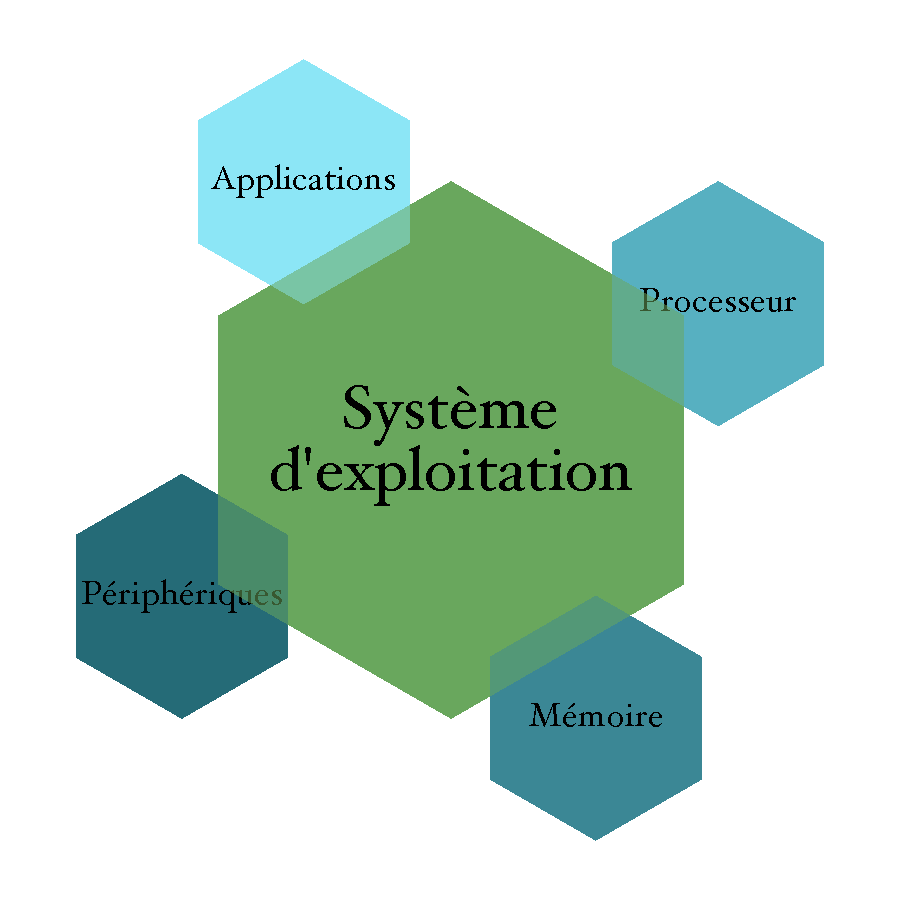
\includegraphics[height=5cm, width=5cm]{textures/images/intro/os.pdf}
\end{minipage}%
\begin{minipage}{7cm}
  Le système d'exploitation est l'\textcolor{blue}{intermédiaire} entre les
logiciels, l'utilisateur et le matériel. \\

  Il gère ainsi la mémoire de l'ordinateur et la répartit entre tous les
programmes. \\

  Par conséquent, lorsqu'une application \\ nécessite diverses informations, il
lui suffit de faire \textcolor{blue}{appel} au système d'exploitation.
\end{minipage}
\end{frame}

\begin{frame}
  \frametitle{Rôles}
  \begin{itemize}
  \item Gestion du processeur

  \item Gestion de la mémoire vive

  \item Gestion des entrées/sorties (\textit{I/O})

  \item Gestion de l'exécution des applications

  \item Gestion des droits

  \item Gestion des fichiers

  \item Gestion des informations

  \item Gestion de l'environnement de bureau

  \item Gestion de la sécurité
  \end{itemize}
\end{frame}

\begin{frame}
  \frametitle{Différents systèmes d'exploitation}
  Il existe un \textcolor{blue}{grand nombre} de systèmes d'exploitation dédiés
à différents matériels (\textit{ordinateur, smartphones et tablettes, cartes à
puces, véhicules, robots, équipement réseau, etc.}).

\hspace{0.5cm}

Chacun ayant une interface et des logiciels \textcolor{blue}{adaptés} au
matériel pour lequel il est développé.

\hspace{0.5cm}

Les deux familles de systèmes d'exploitation les plus
\textcolor{blue}{populaires} sont :

\hspace{0.5cm}

\begin{itemize}
\item Unix : principalement OS X, GNU/Linux, iOS et Android;

\item Windows : détient un \textcolor{blue}{quasi-monopole} sur les ordinateurs
personnels avec près de 90\% de part de marché depuis 15 ans.
\end{itemize}
\end{frame}

\begin{frame}
  \frametitle{Marché des OS}
  Parts de marché des systèmes d'exploitation les plus
\textcolor{blue}{utilisés} par catégorie : \\

\begin{tabular}{p{5cm} p{6.5cm}}
	\begin{itemize}
  \item[$\bullet$] \textbf{Ordinateur} (Jan. 2016) :
    \begin{enumerate}
    \item Windows (\textbf{85,18\%})
    \item Mac OS X (\textbf{9,03\%})
    \item Autres (\textbf{3,81\%})
    \item GNU/Linux (\textbf{1,47\%})
    \item Chrome OS (\textbf{0,51\%})
    \end{enumerate}
	\end{itemize}
	& \begin{itemize}
  \item[$\bullet$] \textbf{Smartphones/tablettes} (2014) :
    \begin{enumerate}
    \item Android (\textbf{85\%})
    \item iOS (\textbf{11\%})
    \item Windows Phone (\textbf{2,5\%})
    \item BlackBerry OS (\textbf{1\%})
    \item Autres (\textbf{0,5\%})
    \end{enumerate}
	\end{itemize}
\end{tabular}
\end{frame}

\begin{frame}
  \frametitle{Marché des OS}

  En ne gardant que les trois systèmes les \textcolor{blue}{plus utilisés} de
chaque catégorie, on obtient ce classement :

\begin{center}
	\begin{tabular} {p{7cm}}
    \centering
		\begin{enumerate}
    \item Windows \textit{PC et Mobile} (\textbf{45,15\%})
    \item Android (\textbf{43,77\%})
    \item iOS (\textbf{5,66\%})
    \item Mac OS X (\textbf{4,66\%})
    \item Linux (\textbf{0,76\%})
		\end{enumerate}
	\end{tabular}
\end{center}
\begin{figure}[!h]
  \vspace*{-1cm}
  \centering
  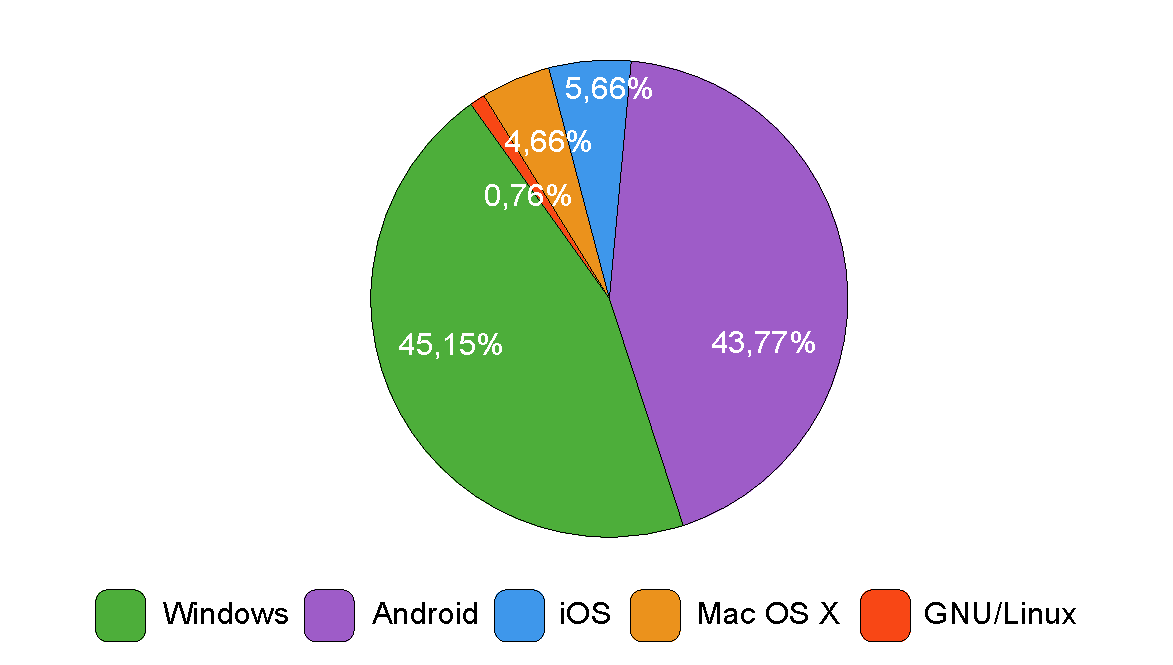
\includegraphics[scale=0.3]
  {textures/images/intro/moreUsedOS.pdf}
\end{figure}
\end{frame}

\begin{frame}
  \frametitle{Marché  des OS}
  Par conséquent, les cinq systèmes d'exploitation les plus utilisés sont, dans
l'ordre \textcolor{blue}{décroissant} :

  \begin{enumerate}
  \item Windows

  \item Android

  \item iOS

  \item Mac OS X

  \item GNU/Linux
  \end{enumerate}

        Il est à noter qu'aux USA, les parts de marché de Windows ont fortement
\textcolor{blue}{baissé} en 8 ans : elles sont passées de près de 95\% à 20\%.

  \hspace{0.5cm}

  Microsoft se retrouve maintenant derrière Google avec Android et Chrome OS
(42\%) et Apple avec OS X et iOS (24\%).
\end{frame}

\begin{frame}
  \frametitle{Marché des OS}
  Logos de ces \textcolor{blue}{différents} systèmes : \\

\begin{columns}
    \begin{column}{0.3 \textwidth}
      \centering
        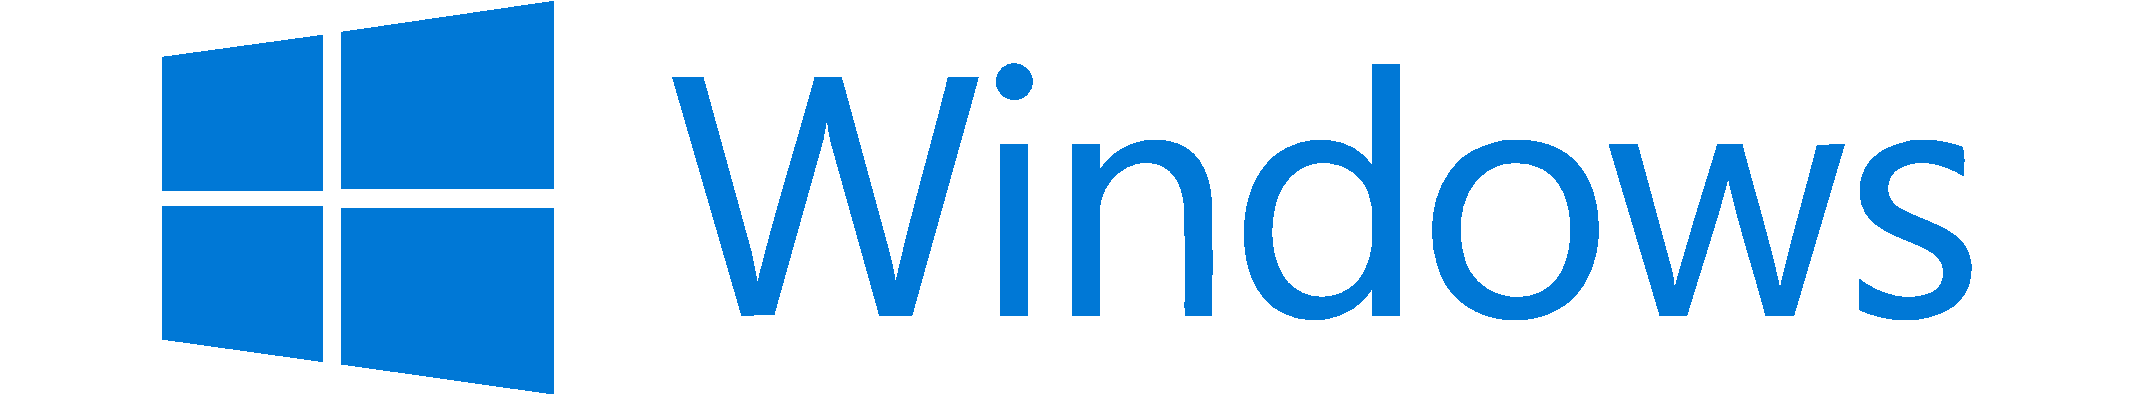
\includegraphics[width=4cm]{textures/images/intro/logo/windows.pdf}\par
      Logo de Windows
    \end{column}
    \begin{column}{0.3 \textwidth}
      \centering
      
\includegraphics[width=1.5cm]{textures/images/intro/logo/android.pdf}\par
      Bugdroid, la mascotte de Android
    \end{column}
    \begin{column}{0.3 \textwidth}
      \centering
              
\includegraphics[width=2cm]{textures/images/intro/logo/ios.pdf}\par
      Logo de iOS
    \end{column}
  \end{columns}
  \begin{columns}
    \begin{column}{0.3 \textwidth}
      \centering
        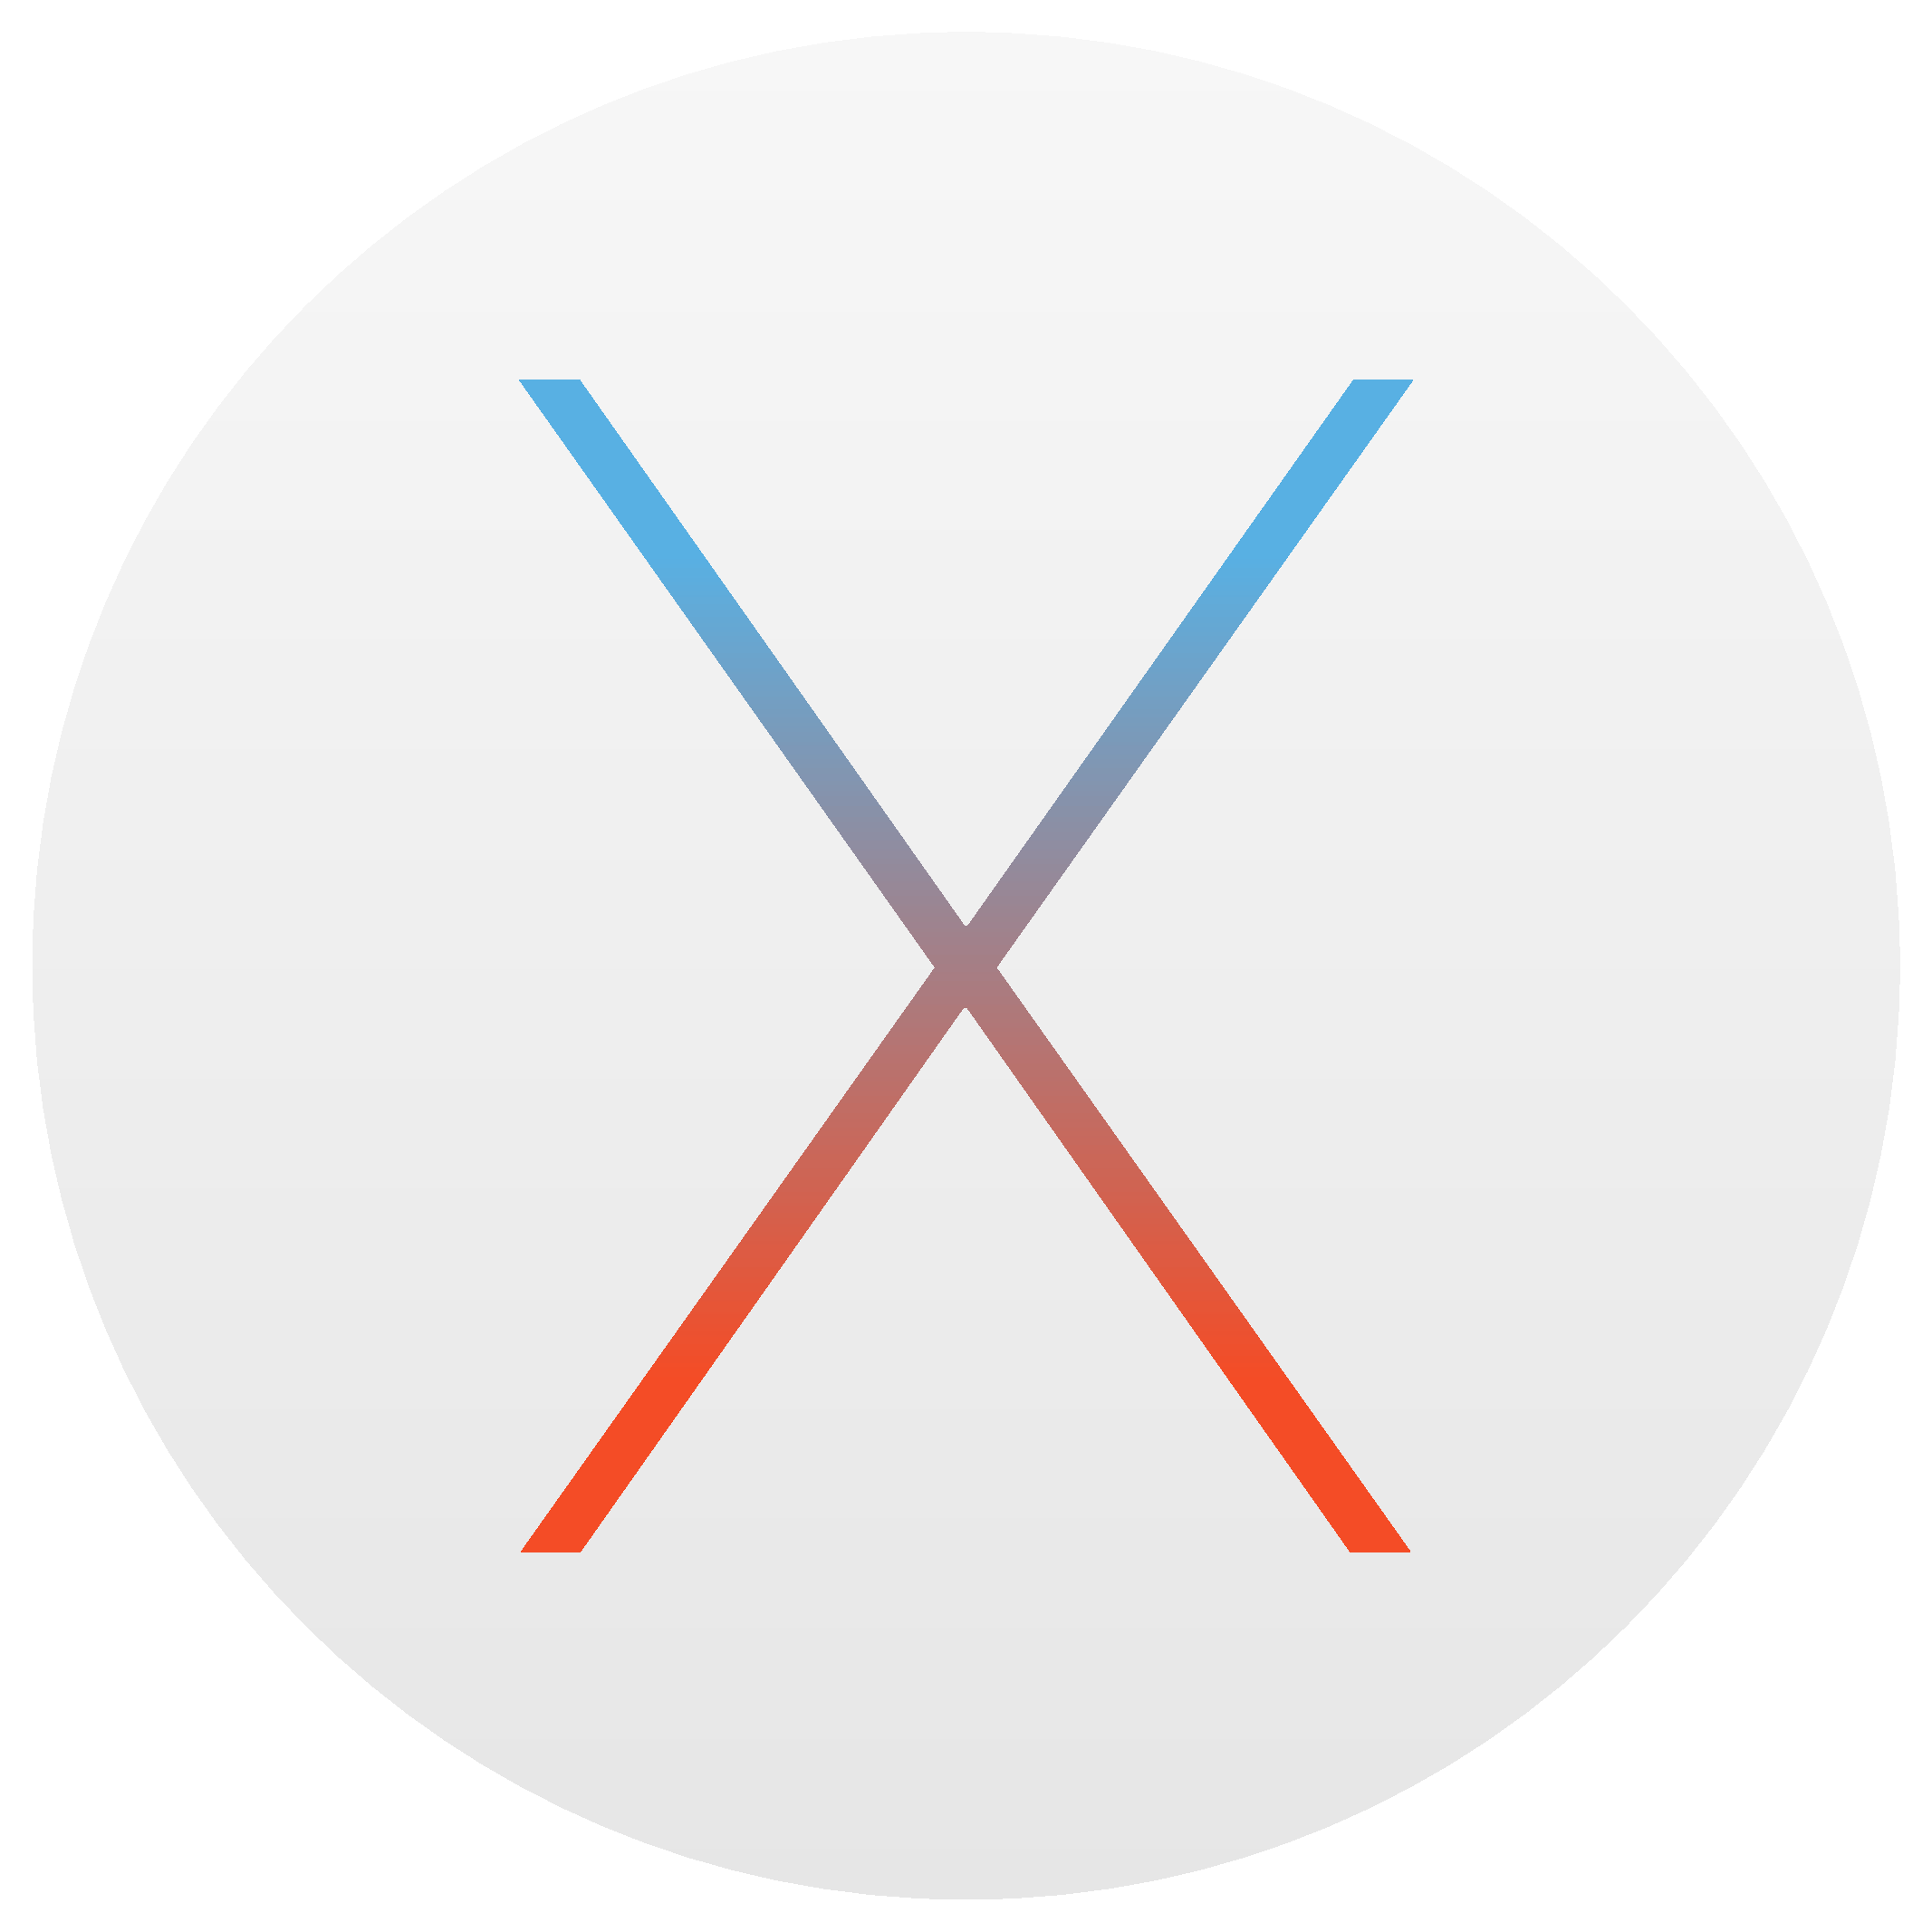
\includegraphics[width=2cm]{textures/images/intro/logo/osx.pdf}\par
      Logo de Mac OS X
    \end{column}
    \begin{column}{0.3 \textwidth}
      \centering
      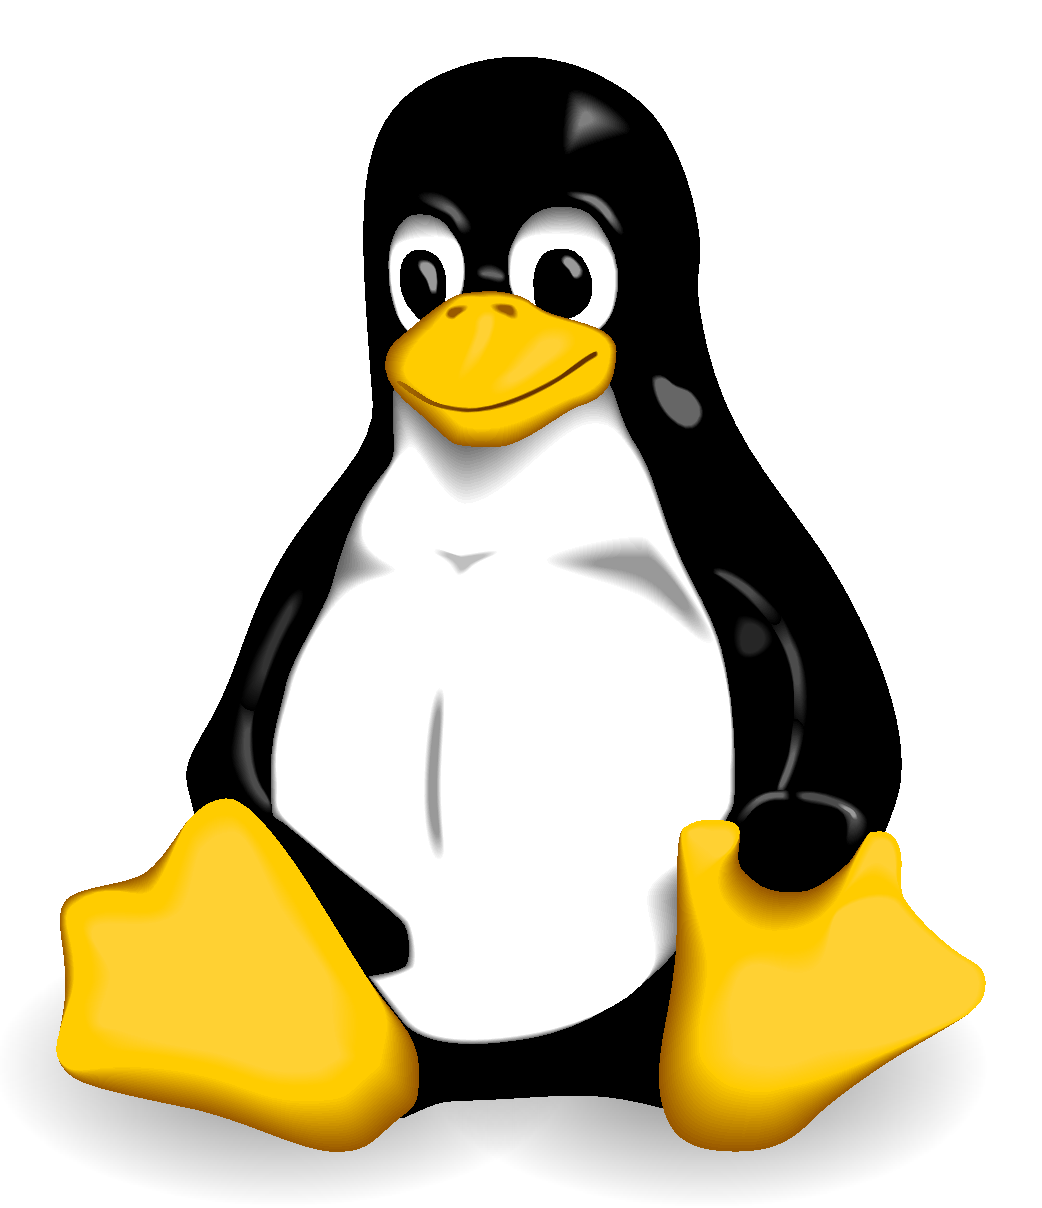
\includegraphics[width=2cm]{textures/images/intro/logo/tux.pdf}\par
      Tux, la mascotte de Linux
    \end{column}
  \end{columns}
\end{frame}

\section{Windows}

\begin{frame}
  \frametitle{Historique}
  Descendant de \textcolor{blue}{MS-DOS} (\textit{Microsoft Disk Operating
    System}) créé en 1981 par Bill Gates, Paul Allen et Steve Ballmer.

  \hspace{0.5cm}

  \begin{columns}
    \begin{column}{0.3 \textwidth}
      \centering
        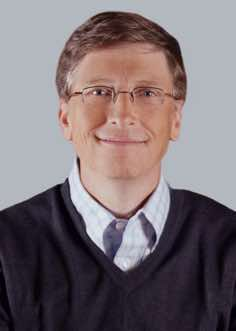
\includegraphics[width=2cm]{textures/images/windows/gates.jpg}\par
      Bill Gates
    \end{column}
    \begin{column}{0.3 \textwidth}
      \centering
      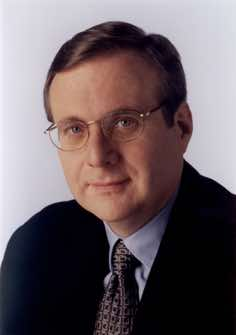
\includegraphics[width=2cm]{textures/images/windows/allen.jpg}\par
      Paul Allen
    \end{column}
    \begin{column}{0.3 \textwidth}
      \centering
              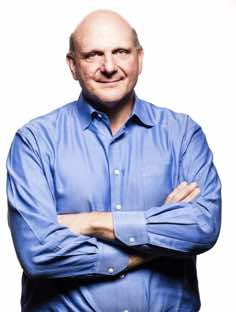
\includegraphics[width=2cm]{textures/images/windows/ballmer.jpg}\par
      Steve Ballmer
    \end{column}
  \end{columns}

\end{frame}

\begin{frame}
  \frametitle{Historique}
  C'est le 20 novembre 1985 qu'apparaît la \textcolor{blue}{première version} de
  \textit{Windows}, \textit{Windows 1.0}, offrant la possibilité
  d'\textcolor{blue}{utiliser} une interface graphique.

  \hspace{0.5cm}

  \textcolor{blue}{20 jours plus tard}, \textit{Windows 2.0} voit le jour offrant la
  possibilité de faire se chevaucher des fenêtres, de contrôler la disposition
  de l'écran ainsi que d'utiliser des raccourcis clavier.

  \hspace{0.5cm}

    En 1988, les ordinateurs commencent à faire partie du
  \textcolor{blue}{quotidien} de divers employés de bureau.
\end{frame}

\begin{frame}
  \frametitle{Historique}
  \textit{Windows 3.0} fut \textcolor{blue}{annoncé} en 1990 et la version 3.1
  sera disponible en 1992.

  \hspace{0.5cm}

  \textit{Windows} \textcolor{blue}{dispose} alors de meilleures performances graphiques
  puisqu'il \textcolor{blue}{supporte} 16 couleurs et s'est amélioré du
  côté des icônes.

  \hspace{0.5cm}

  \textcolor{blue}{Remarque} : \textit{Windows NT}, sorti en juillet 1993, est
  intéressant d'un point de vue \textcolor{blue}{commercial} puisque celui-ci
  est un système d'exploitation 32 bits.
\end{frame}

\begin{frame}
  \frametitle{Historique}
  \textit{Windows 95} sort en août 1995 et offre les fonctionnalités de
  \textcolor{blue}{base} que nous connaissons aujourd'hui (\textit{menu
  démarrer, courrier électronique, jeux multimédias, logiciels éducatifs,...}).

  \hspace{0.5cm}

  À ce moment, 80\% des PC du monde entier \textcolor{blue}{utilisent} \textit{Windows}
  et \textit{MS-DOS}.

  \hspace{0.5cm}

  Juin 1998, \textit{Windows 98} est rendu disponible et devient la première
  version de Windows spécialement \textcolor{blue}{conçue} pour les utilisateurs.

  \hspace{0.5cm}

  Les PC sont dès à présent disponibles tout \textcolor{blue}{autour} de nous,
  que ce soit dans les bureaux, à la maison ou dans des cybercafés.

  \hspace{0.5cm}

  Cette version sera la \textcolor{blue}{dernière} version basée sur \textit{MS-DOS}.
\end{frame}

\begin{frame}
  \frametitle{Historique}
  Toujours dans l'\textcolor{blue}{utilisation} domestique, \textit{Windows} Me
  proposera des perfectionnements pour la musique, la vidéo et le réseau
  domestique, ...

  \hspace{0.5cm}

  Dès lors, Microsoft anonce que tous les prochains systèmes d'exploitaiton
  seront basés sur le \textcolor{blue}{noyau} de \textit{Windows NT} et de \textit{Windows 2000}.

  \hspace{0.5cm}

  \textit{Windows 2000 Professionnel} prend en charge le matériel
  \textcolor{blue}{Plug-and-Play} (\textit{produits sans fil et réseau,
  périphériques USB et infrarouges, etc.}).
\end{frame}

\begin{frame}
  \frametitle{Historique}
  Le très \textcolor{blue}{populaire} \textit{Windows XP} est disponible en octobre 2001
  et est proposé en \textcolor{blue}{plusieurs} versions (\textit{64 bits,
  Media Center, Tablet PC}).

  \hspace{0.5cm}

  Il est fourni dans 25 langues et offre une nouvelle \textcolor{blue}{ergonomie}
  ciblée sur l'utilisation et le centre unifié de services d'aide et d'assistance.

  \hspace{0.5cm}

  En 2006, \textit{Windows Vista} est annoncé, il visera de \textcolor{blue}{renforcer} la
  sécurité (\textit{contrôle de compte d'utilisateur, chiffrement,...}).

  \hspace{0.5cm}

    Néanmoins, cette version de \textit{Windows} fut \textcolor{blue}{beaucoup}
    critiquée (\textit{incompatibilités avec Windows XP, pertes de performance,
    sécurité,…}).
\end{frame}

\begin{frame}
  \frametitle{Historique}
  En 2009, Microsoft introduit l'\textcolor{blue}{interface tactile} à l'aide
  de \textit{Windows 7} vu qu'il est devenu courant de se connecter dans des zones
  d'accès sans fil.

  \hspace{0.5cm}

  Suivant cette direction, \textit{Windows 8}, conçu en 2012, propose une toute
  \textcolor{blue}{nouvelle} interface compatible avec la technologie tactile.

  \hspace{0.5cm}

  Après \textit{Windows 8.1}, vient \textit{Windows 10} qui est le \textcolor{blue}{meilleur}
  \textit{Windows} jamais créé (\textit{sic}).

  \hspace{0.5cm}

  Cette version \textcolor{blue}{dispose} d'une assistante personnelle
  intelligente (\textit{Cortana}).
\end{frame}

\begin{frame}
  \frametitle{Historique}
  \textcolor{blue}{Différentes} versions de \textit{Windows} :

  \begin{figure}[!h]
    \center
    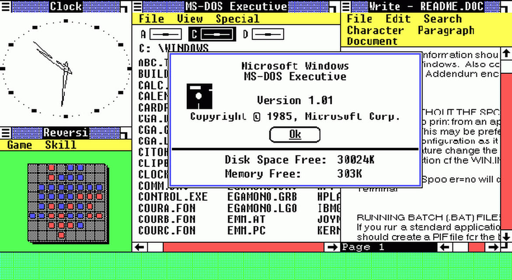
\includegraphics[scale=0.28]
    {textures/images/windows/historic/Win1.png}
    \caption{Windows 1.01}
  \end{figure}
\end{frame}

\begin{frame}
  \frametitle{Historique}
  \begin{figure}[!h]
    \center
    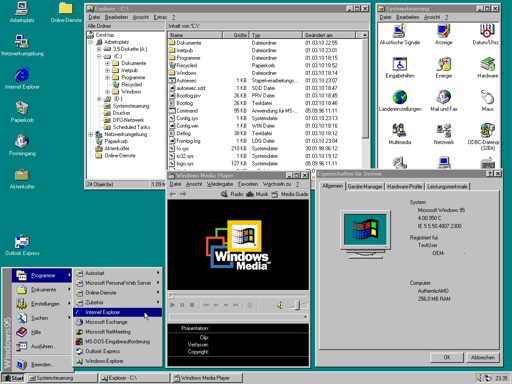
\includegraphics[scale=0.245]
    {textures/images/windows/historic/Win95.png}
    \caption{Windows 95}
  \end{figure}
\end{frame}

\begin{frame}
  \frametitle{Historique}
  \begin{figure}[!h]
    \center
    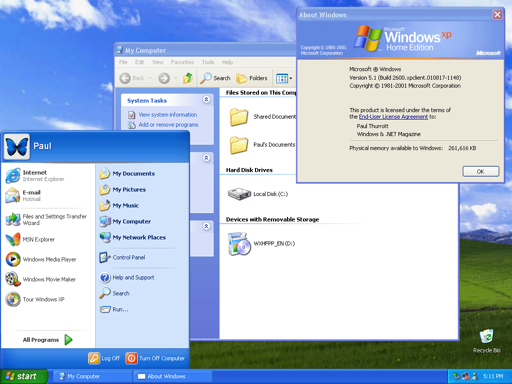
\includegraphics[scale=0.27]
    {textures/images/windows/historic/WinXP.png}
    \caption{Windows XP}
  \end{figure}
\end{frame}

\begin{frame}
  \frametitle{Historique}
  \begin{figure}[!h]
    \center
    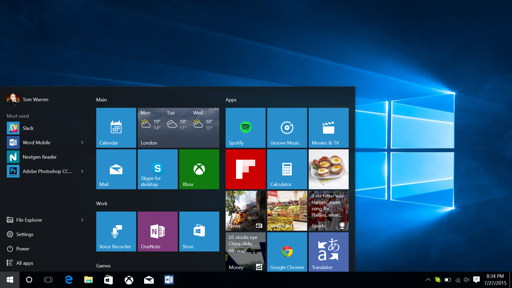
\includegraphics[scale=0.18]
    {textures/images/windows/historic/Win10.png}
    \caption{Windows 10}
  \end{figure}
\end{frame}

\begin{frame}
  \frametitle{Utilisation}
  \textit{Windows} est le \textcolor{blue}{premier} système d'exploitation pour les PC
  en termes de part de marché, il est aisé de savoir le pourquoi du comment de
  cette position.

  \hspace{0.5cm}

    \textit{Windows} est le système d'exploitation installé par \textcolor{blue}{défaut}
    sur tous les ordinateurs.

    \hspace{0.5cm}

    De ce fait, lors de l'achat de l'ordinateur, \textit{Windows} est fourni avec
    celui-ci.

    \hspace{0.5cm}

    Remarque : il est \textcolor{blue}{possible} d'acheter un ordinateur
    directement avec GNU/Linux sur des sites tels que \textit{LDLC} et
    \textit{system76}.
\end{frame}

\begin{frame}
  \frametitle{Utilisation}
  La plupart des développeurs s'occupent en priorité de la
  \textcolor{blue}{compatibilité} sur \textit{Windows} afin de rendre leurs logiciels
  accessibles à un vaste public.

  \hspace{0.5cm}

  \textit{Windows} a également l'avantage de regrouper diverses
  \textcolor{blue}{catégories} de personnes: adolescents, adultes, personnes
  âgées,...

  \hspace{0.5cm}

  \textit{Windows} est donc un système d'exploitation \textcolor{blue}{universel}
  regroupant une large communauté offrant de trouver facilement une réponse à un
  problème ou une question sur l'OS.
\end{frame}

\begin{frame}
  \frametitle{Utilisation}
  Il est également \textcolor{blue}{possible} d'utilier cet OS sur son
  téléphone. Effectivement, des smartphones sont équipés de \textit{Windows Phone}.

  \hspace{0.5cm}

  Même si celui-ci est \textcolor{blue}{moins répandu} qu'Android et iOS, il a
  l'avantage d'être très rapide sur de petites configurations et d'offrir des
  téléphones à prix raisonnable.
\end{frame}

\begin{frame}
  \frametitle{Utilisation}
  Néanmoins, certains spécialistes en la matière considèrent que \textit{Windows Phone}
  n'est \textcolor{blue}{pas rentable} pour Microsoft.

  \hspace{0.5cm}

  La principale \textcolor{blue}{raison} étant que de nombreuses
  applications n'existent que sur Android et/ou sur iOS.

  \hspace{0.5cm}

  Dans ce cas, il pourrait être abandonné dans le futur et les utilisateurs
  devraient \textcolor{blue}{se tourner} vers Android ou iOS.
\end{frame}

\begin{frame}
  \frametitle{Mobile}
  Tout comme Apple, Nokia et Samsung, Microsoft possède une
  \textcolor{blue}{longue} histoire dans le mobile.

  \hspace{0.5cm}

  Entre les PDA, les tablettes et les téléphones, ces firmes ont
  \textcolor{blue}{développé} des systèmes d'exploitation mobiles spécialement
  conçus pour ces appareils.

  \hspace{0.5cm}

  La première version de ce système, \textit{Pocket PC 200}, est
  basée sur une version de \textit{Windows} \textcolor{blue}{spécialement} prévue pour
  des appareils possédant peu de ressources - \textit{Windows CE}.
\end{frame}

\begin{frame}
  \frametitle{Mobile}
  Au fil des ans, le nom devient \textit{Windows Mobile 2003} puis \\
  \textit{Windows Mobile 5}, sur laquelle on \textcolor{blue}{retrouve} une adaptation
  d'Office.

  \hspace{0.5cm}

  Avec la sortie de l'iPhone en 2007 suivi très \textcolor{blue}{rapidement}
  par Samsung, \textit{Windows Mobile} est à la traîne. \\
  \textit{Microsoft} présente alors \textit{Windows Phone 7} au public en 2011.

  \hspace{0.5cm}

  Pendant ce temps, \textit{Windows Mobile 6} a connu de \textcolor{blue}{grands}
  changements afin de rester dans la course.
\end{frame}

\begin{frame}
  \frametitle{Mobile}
  La \textcolor{blue}{dernière} version en date est \textit{Windows 10 Mobile} qui est
  très proche de la version bureau, la politique de Microsoft étant d'avoir un
  seul et unique système d'exploitation pour tous les appareils.

    \begin{figure}[!h]
    \centering
    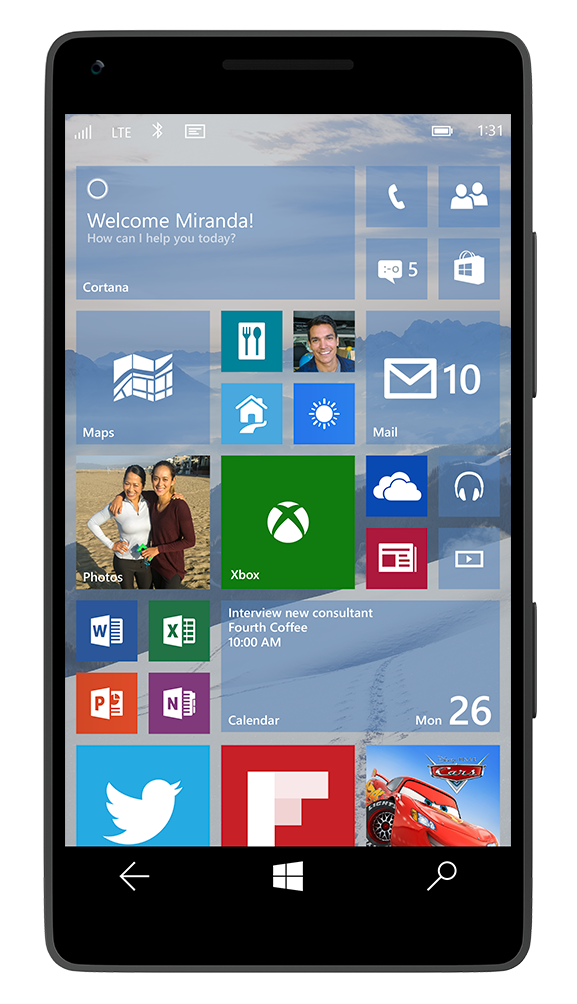
\includegraphics[scale=0.22]
    {textures/images/windows/Windows10Mobile.png}
    \caption{Windows 10 Mobile}
  \end{figure}
\end{frame}

\begin{frame}
  \frametitle{Fonctionnalités}
  Le système d'exploitation de la firme de Redmond possède plusieurs
  \textcolor{blue}{fonctionnalités} bien à lui.

  \hspace{0.5cm}

  Depuis \textit{Windows 10}, les applications \textcolor{blue}{disponibles} dans le
  \textit{Windows Store} sont universelles.

  \hspace{0.5cm}

  Elles peuvent donc \textcolor{blue}{tourner} sur n'importe quel ordinateur ou
  smartphone possédant \textit{Windows 10}, ainsi que sur les \textit{Xbox One} et les
  \textit{HoloLens}.

  \hspace{0.5cm}

  La \textcolor{blue}{suite} \textit{Microsoft Office} est d'ores et déjà universelle.
\end{frame}

\begin{frame}
  \frametitle{Fonctionnalités}
  Une autre \textcolor{blue}{nouveauté} se nomme \textit{Continuum} et consiste
  à "\textcolor{blue}{transformer}" sa tablette tantôt en ordinateur portable,
  tantôt en tablette.

  \hspace{0.5cm}

  L'utilisateur peut \textcolor{blue}{utiliser} sa tablette en tant que PC,
  avec son clavier et une souris, avec la version PC de \textit{Windows 10} ; puis
  l'utiliser en \textit{mode tablette}.

  \hspace{0.5cm}

  Pour les joueurs \textcolor{blue}{possédant} une \textit{Xbox One}, il est possible
  d'y jouer depuis son ordinateur sous \textit{Windows 10}.

  \begin{figure}[!htb] \minipage{0.45\textwidth}
  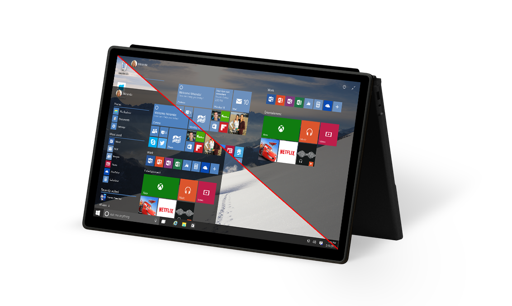
\includegraphics[width=\linewidth]
  {textures/images/windows/features/Continuum_tablet.png}
  \caption{Continuum tablette}\label{fig: Continuum}
	\endminipage\hfill \minipage{0.45\textwidth}
  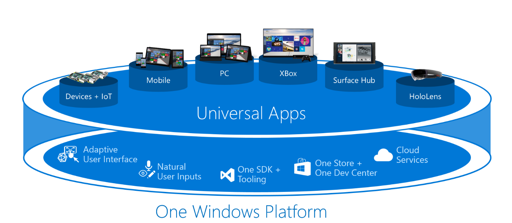
\includegraphics[width=\linewidth]{textures/images/windows/features/Universal_App.png}
  \caption{App universelle}\label{fig:App universelle}
	\endminipage
\end{figure}
  \end{frame}

\section{UNIX}
\begin{frame}
  \frametitle{Historique}
  Créé en 1969 par Ken Thompson et Dennis Ritchie suite à l'idéologie qu'un
système d'exploitation \textcolor{blue}{performant} pour un usage interactif
n'avait nul besoin d'être coûteux, que ce soit en termes d'ordinateur d'accueil
ou de développement humain.

\begin{figure}
\centering
\begin{minipage}{.4\textwidth}
  \centering
  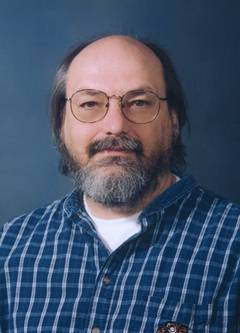
\includegraphics[width=.45\linewidth]{textures/images/unix/thompson.jpeg}
  \caption{Ken Thompson}
\end{minipage}
\begin{minipage}{.45\textwidth}
  \centering
  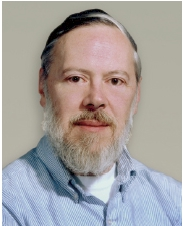
\includegraphics[width=.45\linewidth]{textures/images/unix/ritchie.jpg}
  \caption{Dennis Ritchie}
\end{minipage}
\end{figure}
\end{frame}

\begin{frame}
  \frametitle{Historique}
  Octobre 1973, UNIX commence à prendre sa place au sein du monde informatique,
  les codes sources furent \textcolor{blue}{disponibles} et modifiables par la
  communauté qui apporta à UNIX de meilleurs outils.

\hspace{0.5cm}

Les principales raisons faisant qu'UNIX est encore utilisé aujourd'hui sont
notamment dues à sa \textcolor{blue}{robustesse} et à quelques fonctionnalités
bien élaborées dès sa conception.

\hspace{0.5cm}

De plus, celui-ci possède l'avantage de n'être lié à \textcolor{blue}{aucune}
architecture ni constructeur particulier.
\end{frame}

\begin{frame}
  \frametitle{Historique}
  Il en existe de \textcolor{blue}{nombreuses} versions, y compris les
  \textit{UNIX-like} qui \textcolor{blue}{s'autoproclament} être parfaitement
  compatibles avec UNIX sans avoir la spécification UNIX.

\hspace{0.5cm}

Parmi eux, on retrouve la plupart de systèmes gratuits et/ou open source dont
les plus connus sont \textcolor{blue}{GNU/Linux} et \textcolor{blue}{FreeBSD}.

\hspace{0.5cm}

Ces versions ont l'avantage d'exploiter la \textcolor{blue}{quasi-totalité} du
matériel informatique disponible sur le marché (\textit{serveurs,
super-calculateurs, ordinateurs domestiques, etc.}).
\end{frame}

\begin{frame}
  \frametitle{Historique}
  De même, divers boîtiers réseau (\textit{routeurs, switches,...}) fonctionnent
  sous UNIX et certains ordinateurs de poche (\textit{PDA}) et smartphones sont
  équipés d'UNIX.

\hspace{0.5cm}

Cependant, avant les années 1990, UNIX n'a été disponible que dans le
\textcolor{blue}{monde scientifique} avec une interface utilisateur austère.

\hspace{0.5cm}

Suite à l'apport du protocole graphique \textit{X-Windows} développé par le MIT, tout
utilisateur peut \textcolor{blue}{utiliser} une station \textit{UNIX} à l'aide d'une
souris et d'un écran graphique.
\end{frame}

\begin{frame}
  \frametitle{Historique}
  En 1991, Linus Torvalds - étudiant en informatique à l'Université \\
  d'Helsinki - conçoit le \textcolor{blue}{noyau} Linux.

  \hspace{0.5cm}

  Cela est dû à une déception du système d'exploitation MS-DOS et à cause d'un
manque de bonne \textcolor{blue}{émulation} de terminal proposé par MINIX, un
clone open source d'\textit{UNIX} développé par Andrew Tanenbaum.

\begin{figure}
\centering
\begin{minipage}{.455\textwidth}
  \centering
  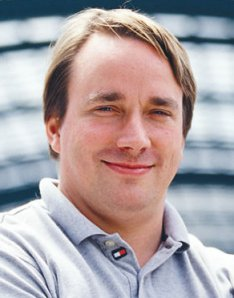
\includegraphics[width=.45\linewidth]{textures/images/unix/torvalds.jpg}
  \caption{Linus Torvalds}
\end{minipage}
\begin{minipage}{.39\textwidth}
  \centering
  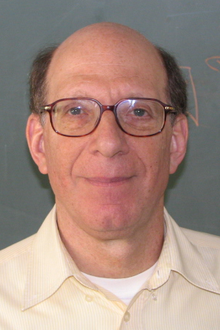
\includegraphics[width=.45\linewidth]{textures/images/unix/tanenbaum.png}
  \caption{Andrew Tanenbaum}
\end{minipage}
\end{figure}
\end{frame}

\begin{frame}
  \frametitle{Composition}
  Le système  d'exploitation \textit{UNIX} \textcolor{blue}{comporte} un ensemble
  d'outils mis à disposition de l'utilisateur.

  \hspace{0.5cm}

  Son rôle principal est la répartition \textcolor{blue}{automatique} des
ressources de manière équitable entre les différentes tâches et utilisateurs.
\end{frame}

\begin{frame}
  \frametitle{Composition}
  \textit{UNIX} est composé des éléments suivant :

  \hspace{0.5cm}

  \begin{itemize}
  \item Un noyau \textcolor{blue}{assurant} la gestion de la mémoire, les
  \textcolor{blue}{échanges} d'entrées/sorties de bas niveau ainsi que la
  \textcolor{blue}{répartition} des tâches.

  \item Un ensemble d'\textcolor{blue}{utilitaires} de base :

    \begin{itemize}
    \item Divers interpréteurs de commande.

    \item Éditeurs de textes (\textit{nano, vim}).

    \item Compilateurs ainsi que des éditeurs de liens.

    \item Outils généraux de développement.

    \item Utilitaires résident (\textit{démons}).
    \end{itemize}
  \end{itemize}
\end{frame}

\begin{frame}
  \frametitle{Composition}

  Par conséquent, \textit{UNIX} peut être vu comme le contenant d'une
  \textcolor{blue}{stratification} en couches.

  \begin{figure}[!h]
    \centering
    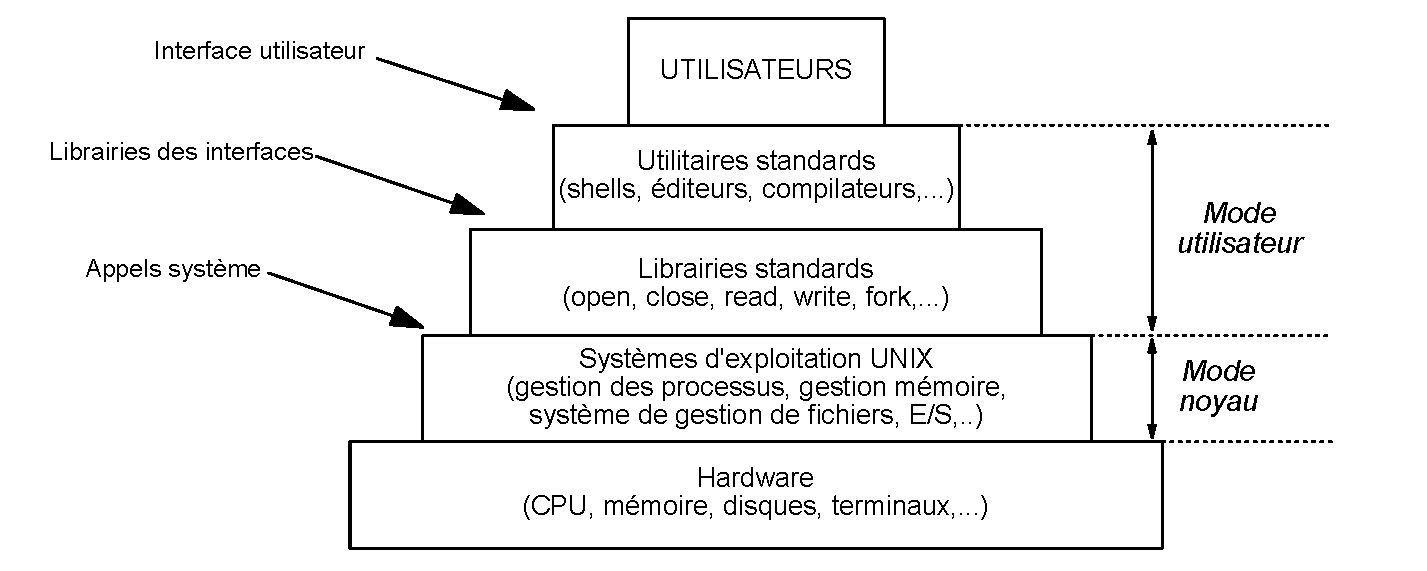
\includegraphics[scale=0.5]
    {textures/images/unix/composition.pdf}
    \caption{Composition d'UNIX}
  \end{figure}
\end{frame}

\begin{frame}
\frametitle{Distributions}
Les distributions sont composées d'un ensemble de logiciels définis en
\textcolor{blue}{fonction} de la distribution choisie et d'un système
d'exploitation comportant un noyau.

\hspace{0.5cm}

Linux en possède un très \textcolor{blue}{grand nombre} en fonction des besoins
de l'utilisateur.

\hspace{0.5cm}

\textcolor{blue}{Attention}, il est important de choisir sa distribution en
fonction de ses \textcolor{blue}{compétences} et de ses
\textcolor{blue}{attentes}.

\hspace{0.5cm}

\end{frame}

\begin{frame}
\frametitle{Distributions}
\textcolor{blue}{Exemples} de distributions : \\

\begin{itemize}
  \item Ubuntu : distribution fournissant un système \textcolor{blue}{convivial}
  et ergonomique pour le grand public.

\begin{center}
    
\includegraphics[scale=0.1]
    {textures/images/unix/logos/ubuntu.pdf}
  \end{center}

    \item Red Hat : distribution orientée \textcolor{blue}{serveurs} et destinée
    à un public professionnel.

\begin{center}
    
\includegraphics[scale=0.2]
    {textures/images/unix/logos/redhat.pdf}
  \end{center}

      \item Debian : probablement la distribution la plus populaire dont les
maîtres mots sont la \textcolor{blue}{stabilité} et
l'\textcolor{blue}{efficacité}
\end{itemize}

\begin{center}
    
\includegraphics[scale=0.3]
    {textures/images/unix/logos/debian.pdf}
\end{center}

\end{frame}

\begin{frame}
\frametitle{Distributions}
\begin{itemize}
  \item Fedora : distribution communautaire de Red Hat dont la caractéristique
première est de suivre les \textcolor{blue}{nouveautés} technologiques.

    \begin{center}
      
\includegraphics[scale=0.2]
      {textures/images/unix/logos/fedora.pdf}
    \end{center}

  \item Arch Linux : comme Debian, cette distribution, fournissant
\textcolor{blue}{peu} d'utilitaires d'aide à la configuration, est destinée aux
utilisateurs avancés.

    \begin{center}
      
\includegraphics[scale=0.6]
      {textures/images/unix/logos/archlinux.pdf}
    \end{center}

  \item Slackware : c'est la plus \textcolor{blue}{vieille} des distributions
    encore utilisées dont l'idéologie est d'être rapide et sans fioritures.
    Celle-ci est principalement utilisée sur des serveurs.

    \begin{center}
      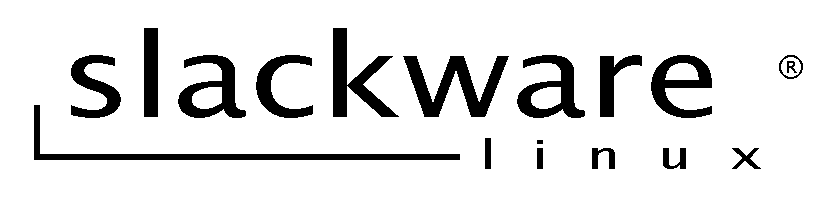
\includegraphics[scale=0.2]
      {textures/images/unix/logos/slackware.pdf}
    \end{center}
\end{itemize}
\end{frame}

\begin{frame}
\frametitle{Environnements de bureau}
À ne \textcolor{blue}{pas confondre} avec le système d'exploitation,
l'environnement de bureau constitue les \textcolor{blue}{caractéristiques
graphiques} du système d'exploitation.

\hspace{0.5cm}

C'est lui qui permet à l'utilisateur d'\textcolor{blue}{interagir}
avec son ordinateur.

\hspace{0.5cm}

Celui-ci est \textcolor{blue}{constitué} de divers éléments :

\begin{itemize}
\item Bureau : \textcolor{blue}{affichage} d'un arrière-plan et d'icônes.

\item Gestionnaire de fenêtres : \textcolor{blue}{délimitations} des fenêtres
par des cadres.

\item Barres de menu et panneaux associés : \textcolor{blue}{accès} aux logiciels,
à l'heure, liste les fenêtres en cours, ...

\item Gestionnaire de session : gère les \textcolor{blue}{sessions} de
l'ordinateur.

\item Outils graphique : permettent de \textcolor{blue}{contrôler}
l'ordinateur.
\end{itemize}
\end{frame}

\begin{frame}
  \frametitle{Environnements de bureau}
  \textcolor{blue}{Exemples} d'environnements de bureau :

  \begin{figure}[!h]
    \center
    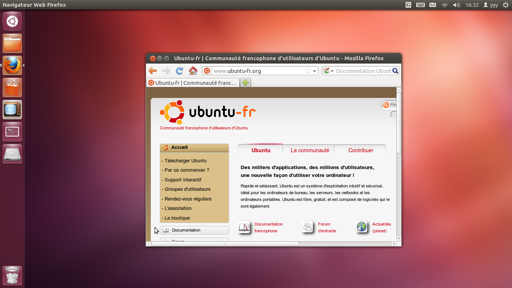
\includegraphics[scale=0.23]
    {textures/images/unix/desktop_environment/unity.png}
    \caption{Unity}
  \end{figure}
\end{frame}

\begin{frame}
  \frametitle{Environnements de bureau}
  \begin{figure}[!h]
    \center
    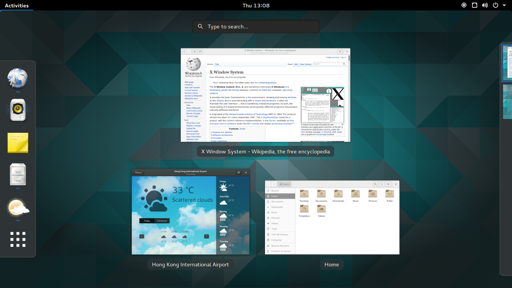
\includegraphics[scale=0.245]
    {textures/images/unix/desktop_environment/gnome-shell.png}
    \caption{Gnome Shell}
  \end{figure}
\end{frame}

\begin{frame}
  \frametitle{Environnements de bureau}
  \begin{figure}[!h]
    \center
    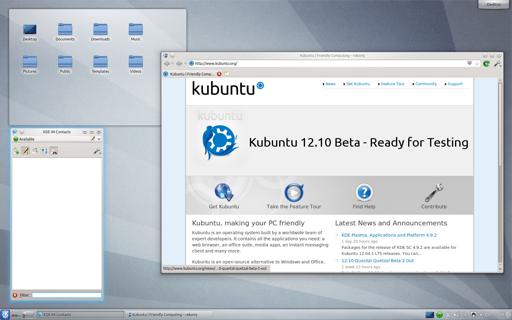
\includegraphics[scale=0.25]
    {textures/images/unix/desktop_environment/kde.png}
    \caption{KDE}
  \end{figure}
\end{frame}

\begin{frame}
  \frametitle{Environnements de bureau}
  \begin{figure}[!h]
    \center
    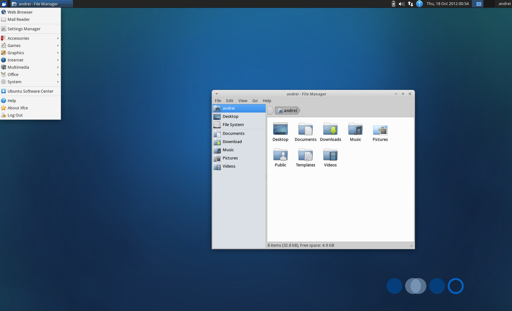
\includegraphics[scale=0.2]
    {textures/images/unix/desktop_environment/xfce.png}
    \caption{XFCE}
  \end{figure}
\end{frame}

\begin{frame}
  \frametitle{Mobilité}
  Chez GNU/Linux, il existe un \textcolor{blue}{grand nombre} de systèmes
  d'exploitation mobiles, et Android en est le plus connu.

  \hspace{0.5cm}

  Pour tout dire, c'est même les \textcolor{blue}{plus utilisé} des systèmes
d'exploitation pour smartphones et tablettes, avec ses 85\% de parts de marché
mobile dans le monde.

  \hspace{0.5cm}

Basé sur un noyau Linux et développé par \textit{Android, Inc.}, il est
\textcolor{blue}{conçu} pour les smartphones et les tablettes.
\end{frame}

\begin{frame}
  \frametitle{Mobilité}
  Le système étant distribué à tout constructeur, Android se trouve être le
\textit{Windows} sur mobile : la \textcolor{blue}{majorité} des mobiles tournant
sous Android.

  \hspace{0.5cm}

Android a gagné en fonctionnalités et peut tourner sur \textcolor{blue}{plus} de
dispositifs, comme des télévisions (\textit{Android TV}), voitures
(\textit{Android Auto}), smartwatches (\textit{Android Wear}), et des ordinateurs
(\textit{Android-x86}).

  \hspace{0.5cm}

Nous en sommes désormais à la \textcolor{blue}{sixième} version, nommée
\textit{Marshmallow}.
\end{frame}

\begin{frame}
\frametitle{Mobilité}
 L'une des \textcolor{blue}{particularités} est que chaque version possède
 un nom de sucrerie et qu'ils se suivent dans l'ordre alphabétique
 (\textit{Cupcake, \textit{Donut}, Eclair} et \textit{Jelly Bean,
 KitKat, etc.}).

  \begin{figure}[!h]
    \centering
    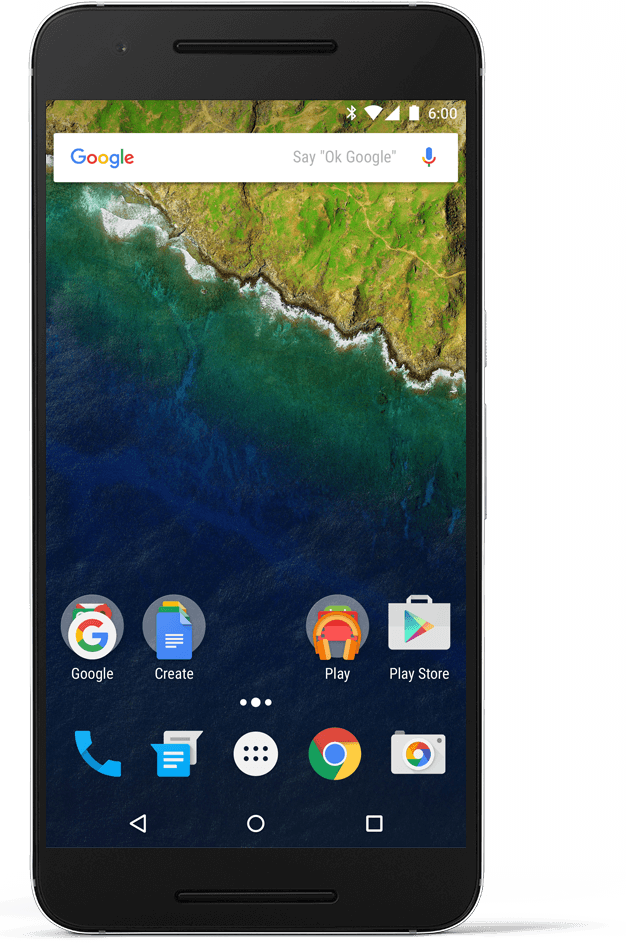
\includegraphics[scale=0.15]
    {textures/images/unix/mobiles/nexus.png}
    \caption{Nexus 6P sous Android 6.0 Marshmallow}
  \end{figure}
\end{frame}

\begin{frame}
\frametitle{Mobilité}
Contrairement aux autres acteurs du marché, GNU/Linux se finance principalement
à l'aide de \textcolor{blue}{donations}, ce qui peut poser des problèmes pour
le financement du développement.

\hspace{0.5cm}

Malgré tout ça, GNU/Linux commence à s'intéresser aux \textcolor{blue}{smartphones}
ainsi qu'aux tablettes. En effet, Ubuntu Touch est un système d'exploitation
développé pour ces dispositifs.

\hspace{0.5cm}

Canonical a d'ailleurs annoncé depuis peu le smartphone « Meizu Pro 5 Ubuntu
Edition » qui est disponible depuis \textcolor{blue}{mars 2016}.
\end{frame}

\begin{frame}
  \frametitle{Mobilité}
Ubuntu Touch a opté pour le \textcolor{blue}{glissement} de doigt sur l'écran.
Un simple glissement du centre de l'écran vers la droite ou la gauche
offre la possibilité de \textcolor{blue}{switcher} entre les applications
principales (\textit{Scopes}).

  \begin{figure}[!h]
    \centering
    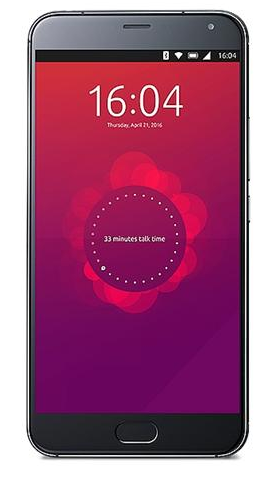
\includegraphics[scale=0.25]
    {textures/images/unix/mobiles/ubuntuTouch.png}
    \caption{Meizu Pro 5 Ubuntu Edition}
  \end{figure}
  \vspace{-3.5mm}

De plus, un glissement partant de la bordure de la dalle tactile ouvre un menu
\textcolor{blue}{multitâches} similaire à celui des concurrents.
\end{frame}

\begin{frame}
  \frametitle{Mobilité}
  Vu que le système d'exploitation est \textcolor{blue}{récent} (\textit{2013}),
  il est difficile de se prononcer sur le succès de celui-ci.

  \hspace{0.5cm}

  Cependant, comme Android occupe la \textcolor{blue}{majorité} du marché et
que celui-ci est composé du noyaux Linux, cela sous-entend que cette
technologie pourrait plaire aux utilisateurs de Android qui désirent une
\textcolor{blue}{nouvelle} interface graphique.
\end{frame}

\section{Mac OS}
\begin{frame}
  \frametitle{Historique}
  C'est en 1976 que le Apple Computer 1, rétroactivement appelé
  \textcolor{blue}{Apple I}, est mis en vente par la \textit{Apple Computer
    Company}  - maintenant appelée \textit{Apple Inc.} et créée le 1er avril 1976.

  \hspace{0.5cm}

  C'est alors l'un des \textcolor{blue}{tout premiers} micro-ordinateurs
  individuels.

  \begin{figure}[!h]
    \centering
    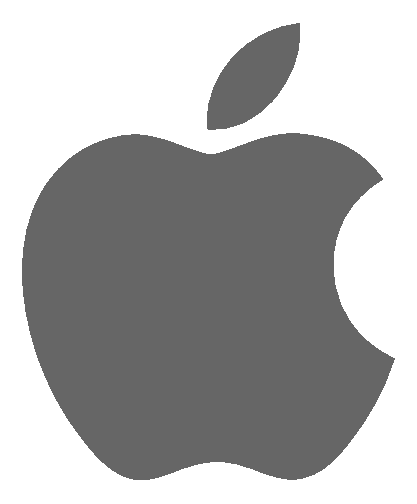
\includegraphics[scale=0.3]
    {textures/images/mac/historic/logo_apple.pdf}
    \caption{Logo actuel de Apple}
  \end{figure}
\end{frame}

\begin{frame}
  \frametitle{Historique}
  Alors que Steve Jobs en fait la publicité, il est construit à la main par
  Steve Wozniak qui en créa le \textcolor{blue}{langage assembleur} en BASIC
  (\textit{en ne passant que par de l'hexadécimal}) afin de pouvoir programmer
  des jeux et y jouer.

  \begin{figure}
  \centering
  \begin{minipage}{.455\textwidth}
    \centering
    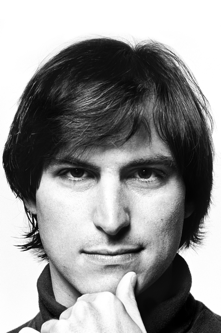
\includegraphics[width=.33\linewidth]{textures/images/mac/jobs.png}
    \caption{Steve Jobs}
  \end{minipage}
  \begin{minipage}{.39\textwidth}
    \centering
    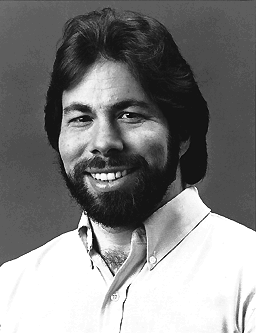
\includegraphics[width=.47\linewidth]{textures/images/mac/wozniak.png}
    \caption{Steve Wozniak}
  \end{minipage}
  \end{figure}
\end{frame}

\begin{frame}
  \frametitle{Historique}
  Les deux premiers ordinateurs avaient un gros \textcolor{blue}{inconvénient}
  : les utilisateurs devaient stocker leurs données sur des
  \textcolor{blue}{cassettes}, ce qui était très lent, incommode et peu fiable.

    \hspace{0.5cm}

  Le DOS 3.1 (\textit{Disk Operating System}) \textcolor{blue}{règle} ce
  problème en permettant d’utiliser des disques durs et des disquettes comme
  périphériques de stockage.
\end{frame}

\begin{frame}
  \frametitle{Historique}
  La même année, sort l'\textcolor{blue}{Apple III} accompagné du SOS
  (\textit{Sophisticated Operating System}).

  \hspace{0.5cm}

  C'est le premier OS pour \textcolor{blue}{micro-ordinateur} à utiliser le
  concept de driver qui aident l’ordinateur à communiquer avec les
  périphériques, ce qui lui offrit une flexibilité à utiliser de nouvelles
  technologies.
\end{frame}

\begin{frame}
  \frametitle{Historique}
  En 1983, le Lisa sort avec le \textcolor{blue}{Lisa OS} qui prend en charge
  le multitâche et la protection de mémoire (\textit{droit d’accès à la mémoire
    non allouée}).

    \hspace{0.5cm}

    Après cela, vient le \textcolor{blue}{Macintosh} avec le System 1.

    \hspace{0.5cm}

    Les premiers \textcolor{blue}{Macintosh} ont
    utilisé des versions successives du \textit{Système} numérotées de 1 à 7.

    \hspace{0.5cm}

    C’est
    à partir de la version 7.6 qu’il prend le nom de \textit{Mac OS}.

    \hspace{0.5cm}

    La version actuelle étant la \textcolor{blue}{dixième} version majeure
    ainsi que la version \textit{UNIX} du système, son nom est devenu Mac OS X
    (\textit{Mac OS Ten}).
\end{frame}

\begin{frame}
  \frametitle{Historique}
  En effet, c'est depuis 1999 et le premier \textcolor{blue}{iMac} que le
  système d'exploitation des ordinateurs Apple est Mac OS X. C'est la
  \textcolor{blue}{fusion} entre Mac OS et NeXTSTEP, un \textit{UNIX-like} basé sur un
  noyau Mach et sur l’implémentation BSD d’\textit{UNIX}.

  \hspace{0.5cm}

  Depuis la version 10.5 (en 2007), le système d’exploitation possède la
  \textcolor{blue}{certification} \textit{UNIX}.
\end{frame}

\begin{frame}
  \frametitle{Historique}
  Différents \textcolor{blue}{systèmes} d'Apple :

  \begin{figure}[!h]
    \center
    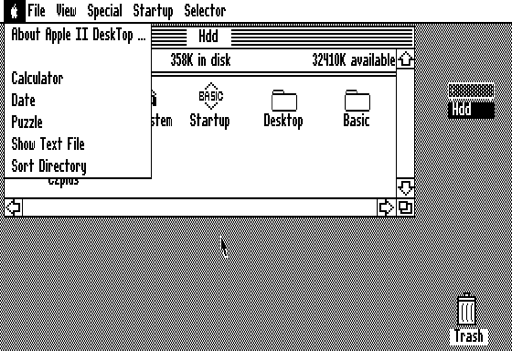
\includegraphics[scale=0.48]
    {textures/images/mac/historic/apple2.png}
    \caption{Apple II Desktop}
  \end{figure}
\end{frame}

\begin{frame}
  \frametitle{Historique}
  \begin{figure}[!h]
    \center
    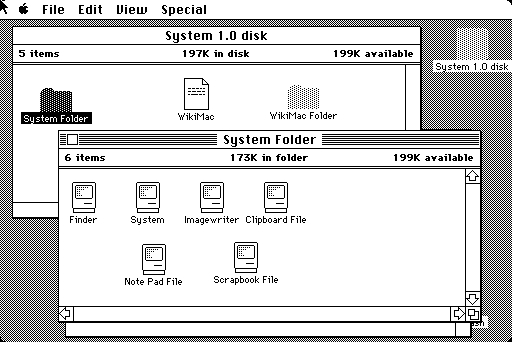
\includegraphics[scale=0.59]
    {textures/images/mac/historic/system1.png}
    \caption{System 1}
  \end{figure}
\end{frame}

\begin{frame}
  \frametitle{Historique}
  \begin{figure}[!h]
    \center
    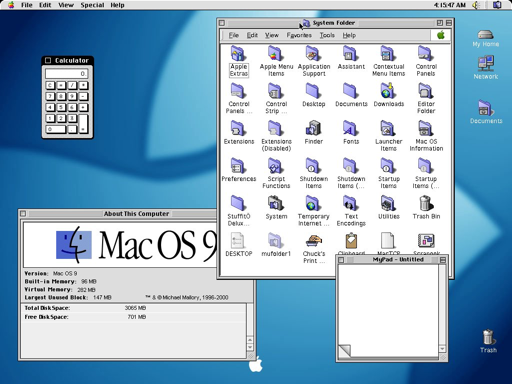
\includegraphics[scale=0.35]
    {textures/images/mac/historic/macos9.png}
    \caption{Mac OS 9}
  \end{figure}
\end{frame}

\begin{frame}
  \frametitle{Historique}
  \begin{figure}[!h]
    \center
    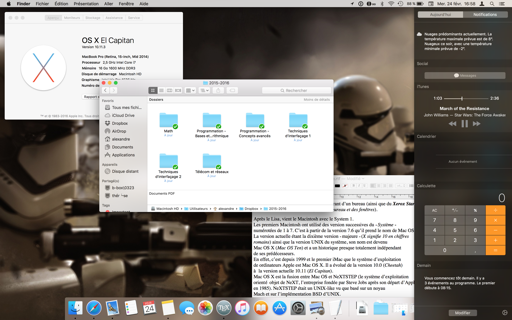
\includegraphics[scale=0.18]
    {textures/images/mac/historic/macosx11.png}
    \caption{Mac OS X 10.11}
  \end{figure}
\end{frame}

\begin{frame}
  \frametitle{Dérivés}
  Peu connu du grand public, \textit{Mac OS X Server} est
  \textcolor{blue}{téléchargeable} sur tout mac et prend la forme d’une
  \textcolor{blue}{simple} application qui permet de gérer facilement des
  ordinateurs, calendriers, fichiers, sauvegardes, etc.

  \hspace{0.5cm}

  Apple possède encore trois autres systèmes d’exploitation basés sur OS X:
  \\ watchOS pour l’Apple Watch, tvOS pour l’Apple TV  et iOS pour les
  \textit{iDevices} (iPhone, iPad et iPod Touch).
\end{frame}

\begin{frame}
  \frametitle{Dérivés}
  Son nom vient de \textcolor{blue}{iPhoneOS} devenu iOS en 2010, lors de la
  sortie du premier iPad.
  % Expliquer à l'oral
  \begin{figure}[!h]
    \center
    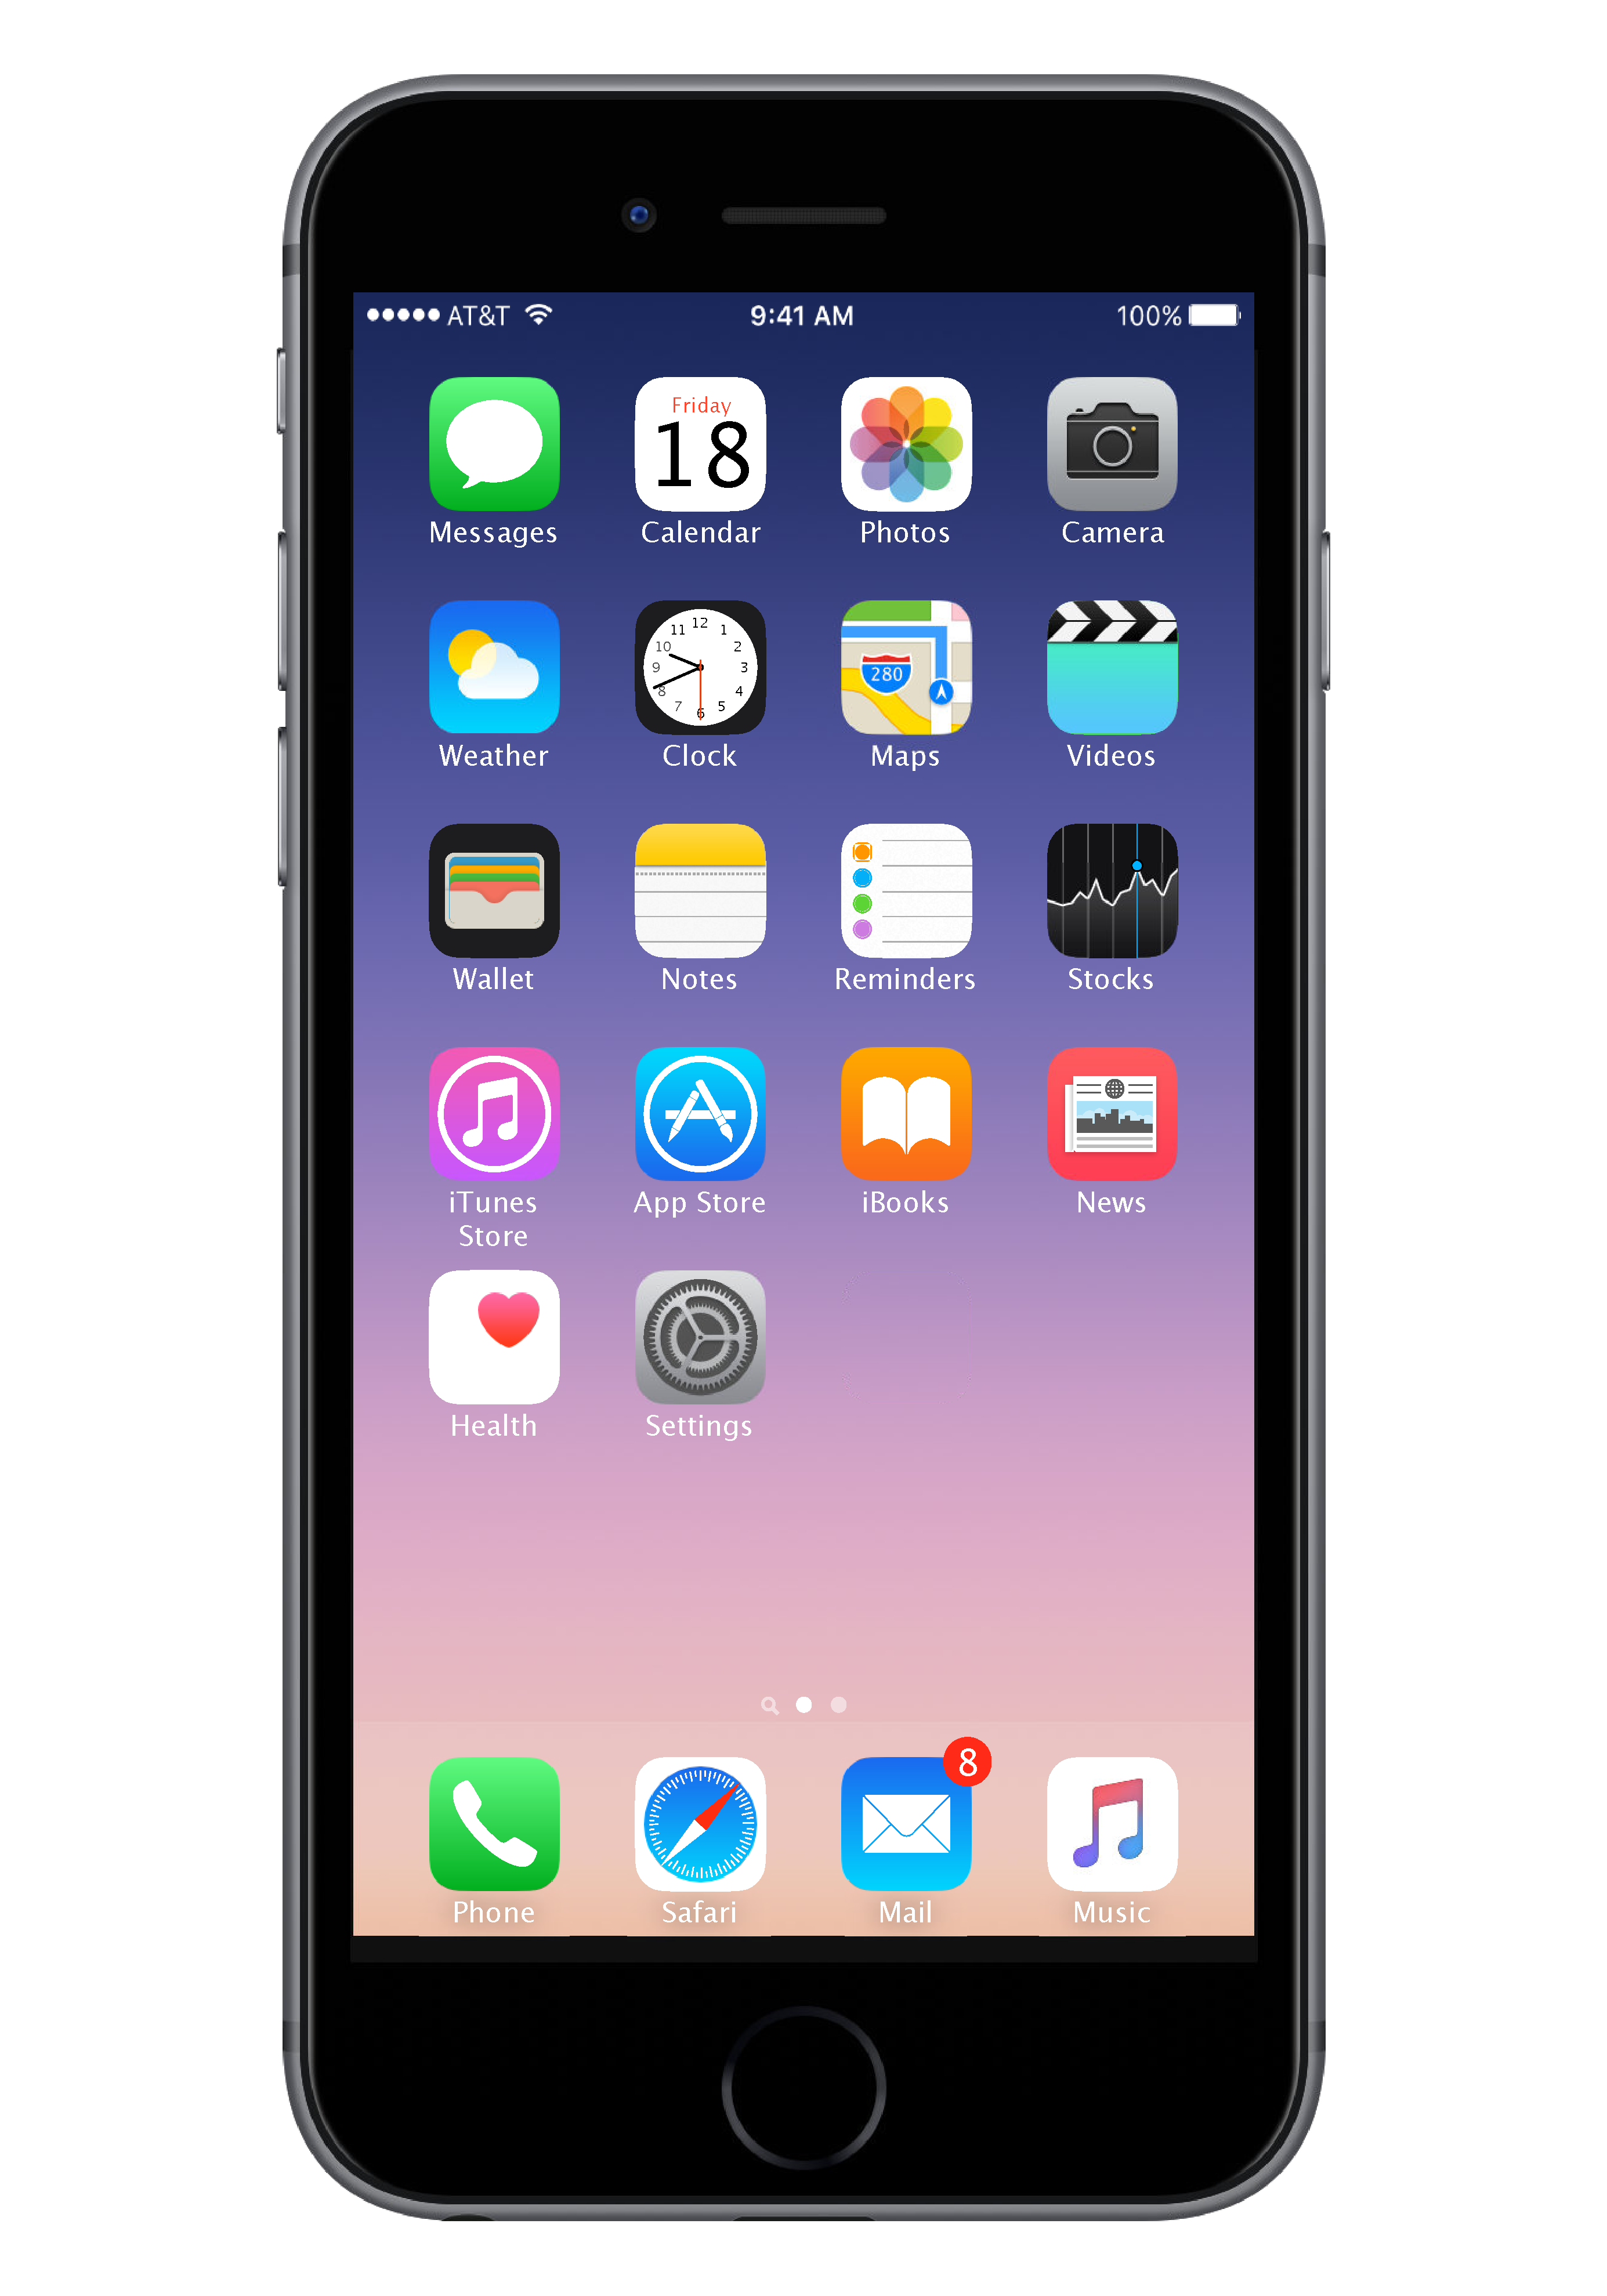
\includegraphics[scale=0.08]
    {textures/images/mac/historic/iOS.pdf}
    \caption{Système d'exploitation iOS}
  \end{figure}
\end{frame}

\begin{frame}
  \frametitle{Popularité}
  Les \textcolor{blue}{avis} à l’encontre de Mac OS X sont assez partagés.

  \hspace{0.5cm}

  Les détracteurs pointent du doigt le prix fort \textcolor{blue}{élevé} à
  l’achat ainsi que la presque impossibilité de mise à jour matérielle des
  macs. \\
  Par contre, ces personnes ont parfois une vision \textcolor{blue}{biaisée} à
  propos de OS X. (\textit{fonctions basiques payantes, système limité,…})

  \hspace{0.5cm}

  Les partisans mettent en avant la \textcolor{blue}{stabilité}, la sécurité,
  la fiabilité et la vitesse de l’OS.

  \hspace{0.5cm}

  La \textcolor{blue}{facilité} d’utilisation étant une des forces des systèmes
  d’Apple, ainsi que sa base \textit{UNIX} offrant la \textcolor{blue}{puissance} de la
  ligne de commande au système.
\end{frame}

\begin{frame}
  \frametitle{Popularité}

  L’augmentation des parts de marché des macs est
  \textcolor{blue}{principalement} due aux iPods, aux iPhones et aux iPads.

  \hspace{0.5cm}

  Avoir un ou des iDevices et un mac crée un \textcolor{blue}{écosystème} : il
  y a un gain de fonctionnalités et passer de l’un à un l’autre n'est pas
  dépaysant.

  \hspace{0.5cm}

  OS X possède de \textcolor{blue}{nombreuses} fonctionnalités et applications préinstallées et
  d'autres sont disponibles comme \textit{Xcode, iWork,…}.
\end{frame}

\begin{frame}
  \frametitle{Fonctionnalités}
  Apple a un avantage sur ses concurrents: l'entreprise
  \textcolor{blue}{développe} l'hardware et le software pour qu'ils
  fonctionnent en adéquation. Grâce à cela, Apple peut sortir des sentiers
  battus et exploiter de nouvelles technologies (\textit{trackpad multitouch,
    Thunderbolt,…}).

  \hspace{0.5cm}

  Avec la sortie du \textit{Surface Book}, Microsoft se met au niveau d'Apple
  et 'gagne' un \textcolor{blue}{avantage} par rapport à ses «
  \textit{concurrents} » sur Windows: \\ l'ordinateur est créé en parallèle
  avec le système d'exploitation.
\end{frame}

\begin{frame}
  \frametitle{Fonctionnalités}
  Quelques \textcolor{blue}{fonctionnalités} logicielles exclusives : \\

  \begin{itemize}
  \item \textbf{Quick Look}; \\

  \item \textbf{Time Machine}; \\

  \item \textbf{AirDrop}; \\

  \item \textbf{Handoff}; \\

  \item \textbf{Continuity}; \\

  \item \textbf{Raccourcis}. \\
  \end{itemize}
\end{frame}

\begin{frame}
  \frametitle{Fonctionnalités}
  \begin{figure}[!h]
    \center
    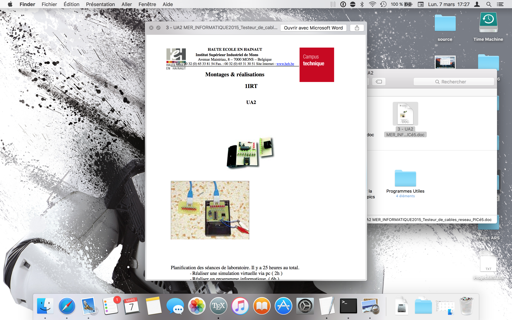
\includegraphics[scale=0.22]
    {textures/images/mac/features/QuickLook.png}
    \caption{QuickLook}
  \end{figure}
\end{frame}

\begin{frame}
  \frametitle{Fonctionnalités}
  \begin{figure}[!h]
    \center
    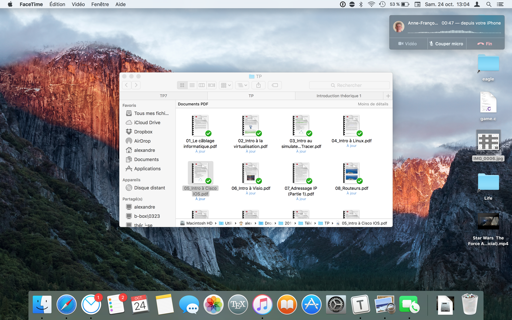
\includegraphics[scale=0.22]
    {textures/images/mac/features/Phone.png}
    \caption{Téléphone}
  \end{figure}
\end{frame}

\begin{frame}
  \frametitle{Fonctionnalités}
  \begin{figure}[!h]
    \center
    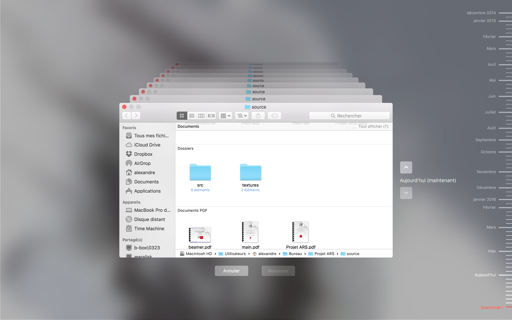
\includegraphics[scale=0.22]
    {textures/images/mac/features/TimeMachine.png}
    \caption{Time Machine}
  \end{figure}
\end{frame}

\begin{frame}
  \frametitle{Fonctionnalités}
  Mac OS X ayant un noyau \textit{UNIX}, l'utilisation du terminal y est à peu près
  \textcolor{blue}{identique} à celle sur Linux.

  \hspace{0.5cm}

  De plus, certains langages de programmation y sont déjà
  \textcolor{blue}{préinstallé} comme Java, Python, Ruby,…
\end{frame}

\section{Autres systèmes}
\begin{frame}
  \frametitle{Les oubliés}
  Il existe de \textcolor{blue}{nombreux systèmes} d'exploitation qui nous
  sont, en partie, \textcolor{blue}{inconnus}.

  \hspace{0.5cm}

  Les systèmes d'exploitation que nous connaissons se sont développés sur base
  de système d'exploitation \textcolor{blue}{expérimentaux} qui ne sont plus utilisés.

  \hspace{0.5cm}

  Exemple :

  \begin{itemize}
  \item Singularity : utilisé pour les recherches de Microsoft;

  \item MyOS : mini système d'exploitation créé à l'aide du langage C++;

  \item Desert Spring-Time (\textit{DST}) : système d'exploitation développé en Objective Caml;

  \item Kid Operating System (\textit{KOS}) : utilisé pour l'apprentissage;

    \item (\textbf{...})
    \end{itemize}
\end{frame}

\begin{frame}
  \frametitle{Les oubliés}
  En outre, il y a des systèmes d'exploitation pour smartphone qui ont été mis
  de côté suite à l'abandon de leur développement au \textcolor{blue}{profit}
  d'autres technologies.

  \hspace{0.5cm}

  Exemple :

  \begin{itemize}
  \item Symbian : développé par Nokia;

  \item Meego : développé par Nokia et Intel;

  \item BlackberryOS : développé par Research In Motion;

  \item Bada : développé par Samsung;

  \item (\textbf{...})
  \end{itemize}
\end{frame}

\begin{frame}
  \frametitle{Les oubliés}
  La majorité des appareils électriques ont un système d'exploitation nommé
  \textcolor{blue}{système embarqué}.

  \hspace{0.5cm}

  Il permet de \textcolor{blue}{gérer} l'aspect informatique du
  composant et offre une interface graphique \textcolor{blue}{conviviale} pour
  interagir avec ces appareils.

  \hspace{0.5cm}

  Par exemple, il en existe pour la télévision :

  \begin{itemize}
  \item Tizen : développé par Samsung;

  \item WebOS : développé par LG;

  \item tvOS : développé par Apple;

  \item Android TV : développé par Google;

  \item (\textbf{...})
  \end{itemize}
\end{frame}

\begin{frame}
  \frametitle{Les oubliés}
  Les voitures et les camions possèdent un ordinateur intégré qui les contrôlent,
  comme l'ABS qui est contrôlé par
  l'ordinateur de bord.

  \hspace{0.5cm}

  L'un des plus gros \textcolor{blue}{problèmes} est la sécurité: on peut
  \textcolor{blue}{pirater} une voiture pour couper son moteur qui sera alors
  impossible à redémarrer.

  \hspace{0.5cm}

  Ce qu'il faudrait, c'est \textcolor{blue}{mettre à jour} le système, un peu
  comme les \textit{Tesla}s qui reçoivent des mises à jour par Internet. \\
  Néanmoins, le procédé n'est pas encore assez fiable...
\end{frame}

\begin{frame}
  \frametitle{Cisco IOS}
  Cisco IOS (\textit{Internetwork Operating System}) est le leader mondial des
  systèmes d'exploitation de réseau, il est développé par \textit{Cisco Systems}
  et équipe la plupart de leurs équipements.

  \begin{figure}[!h]
    \center
    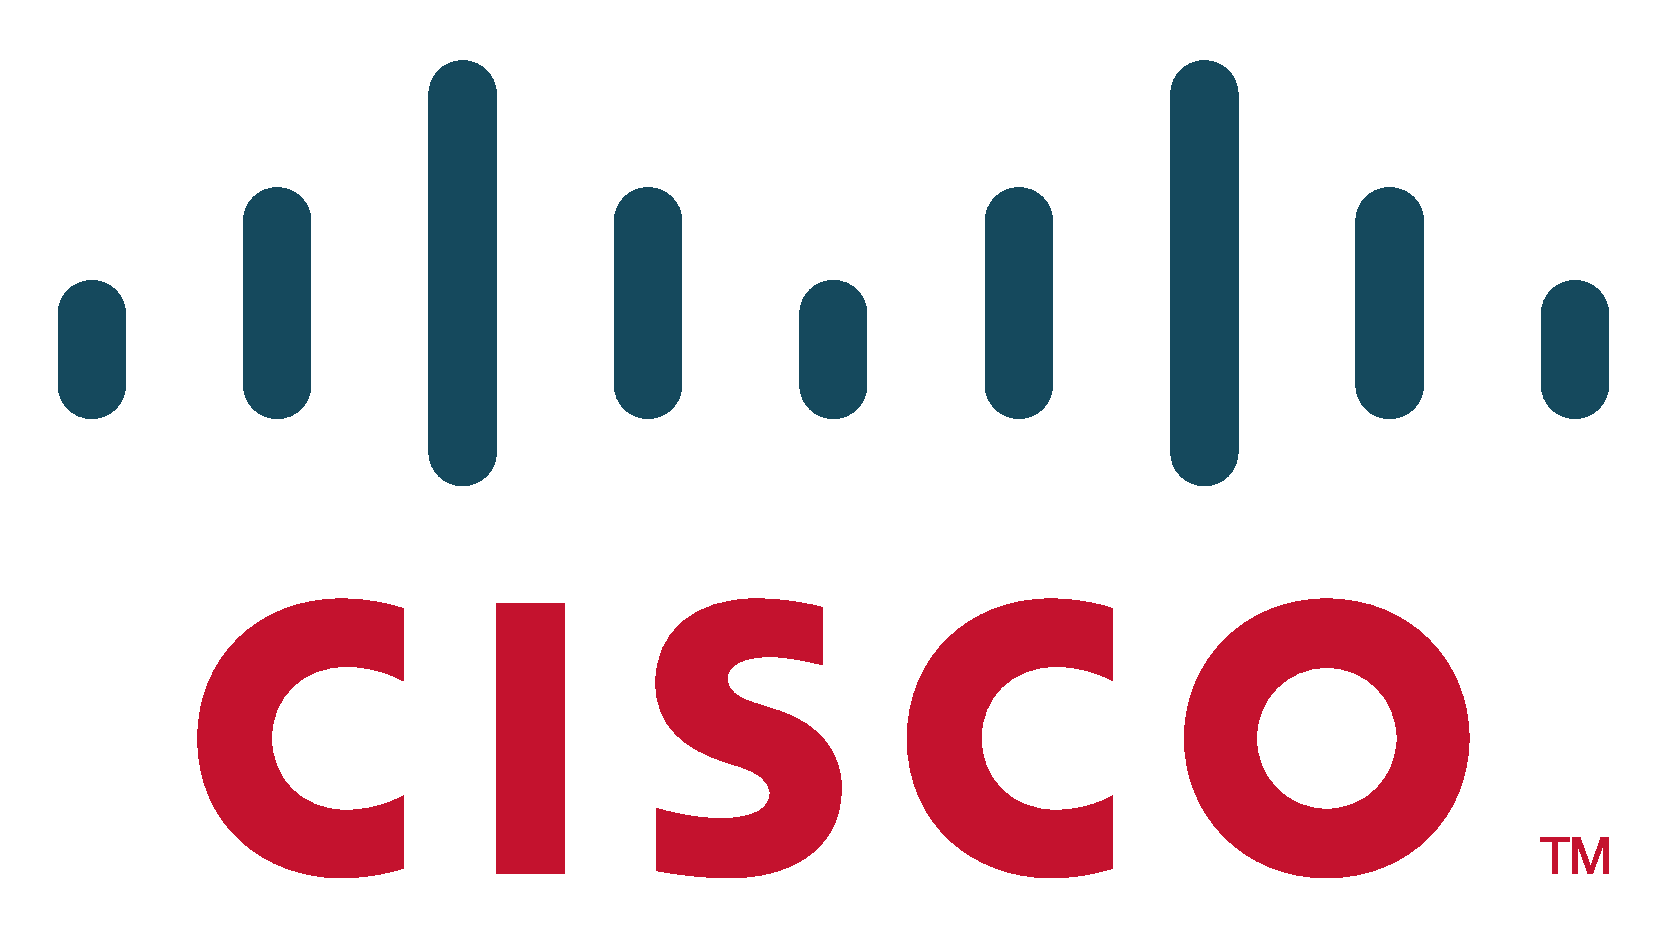
\includegraphics[scale=0.2]
    {textures/images/others/Cisco_logo.pdf}
    \caption{Logo de Cisco Systems}
  \end{figure}

  Il est décliné en différentes versions spécialisées pour chaque équipement
  (\textit{routeur, commutateur, points d’accès Wi-Fi,…}).
\end{frame}

\begin{frame}
  \frametitle{Cisco IOS}
  L’accès se fait par le port console (ou auxiliaire), Telnet ou SSH, et en
  ligne de commande (\textbf{CLI}) ou par une interface web.

  \hspace{0.5cm}

  Du côté de la sécurité, l’accès au périphérique et l’accès au mode d’exécution
  privilégié peuvent être protégé par un mot de passe de même.

  \hspace{0.5cm}

  En effet, il existe plusieurs modes d’exécution:
  \begin{enumerate}
    \item le mode d’exécution utilisateur;
    \item le mode d’exécution privilégié;
    \item le mode de configuration globale;
    \item les autres sous-modes.
  \end{enumerate}

\end{frame}

\begin{frame}
  \frametitle{Cisco IOS}
  Il existe d’autres systèmes d’exploitation de Cisco.

  \hspace{0.5cm}

  Par exemple:
  \begin{itemize}
    \item CatOS : répandu dans les commutateurs Ethernet haut de gamme;
    \item IOS XE : basé sur Linux et compatible avec IOS;
    \item NX-OS : pour les commutateurs Ethernet Nexus et les commutateurs à
      fibre optique MDS.
  \end{itemize}

\end{frame}

\section{Conclusion}

\begin{frame}
  \frametitle{Futur}
  Selon les statistiques, les parts du marché de Windows sont en
  \textcolor{blue}{baisse} suite à l'augmentation de
  l'\textcolor{blue}{utilisation} des périphériques mobiles.

  \hspace{0.5cm}

  Cela annonce le possible \textcolor{blue}{remplacement} des ordinateurs par
  des smartphones et tablettes de plus en plus puissantes.

  \hspace{0.5cm}

  Néanmoins, \textit{Microsoft} a déjà annoncé son \textcolor{blue}{futur}
  système d'exploitation : \textit{Midori}, provenant de \textit{Singularity},
  s'installerait dans une \textcolor{blue}{interface Web}.
\end{frame}

\begin{frame}
  \frametitle{Futur}
  Malgré cela, plusieurs avis \textcolor{blue}{divergent} à propos de l'avenir
  de l'OS.

  Concernant un \textcolor{blue}{futur proche}, certains pensent que l'avenir se
  trouve du côté du \textit{cloud computing} offrant un
  \textcolor{blue}{espace client} avec des composants clés dont les systèmes
  secondaires seront diffusés, chargés ou enlevés.

  \hspace{0.5cm}

  Un tel système nécessitera \textcolor{blue}{fiabilité} et une quasi-constante
  accessibilité des services de \textcolor{blue}{haute vitesse}.

  \hspace{0.5cm}

  Néanmoins, il faudrait y apporter diverses modifications pour le
  \textcolor{blue}{coût} de la bande passante.
\end{frame}

\begin{frame}
  \frametitle{Futur}
  D'autres, estiment que le futur est dans l'\textcolor{blue}{association}
  de Linux et de \textit{Docker}.

  \hspace{0.5cm}

  Ensuite, pour un \textcolor{blue}{futur} à plus \textcolor{blue}{long terme},
  nous nous dirigeons vers les ordinateur \textcolor{blue}{quantiques}, l'idée
  de l'OS sera alors radicalement différente.

  \hspace{0.5cm}

  De ce fait, le calcul sera partagé par de nombreux appareils
  \textcolor{blue}{synchronisés}, et les périphériques
  d'entrées/sorties correspondront à chaque \textcolor{blue}{surface plane},
  comme des claviers projetables sensibles à l'\textcolor{blue}{infrarouge}.

  \hspace{0.5cm}

  Par conséquent, dans un tel environnement informatique, un système
  d'exploitation à base de dispositifs uniques sera
  \textcolor{blue}{obosolète}.
\end{frame}

\begin{frame}
  \frametitle{Futur}
  Ce que l'on peut retenir globalement, c'est qu'il est fort probable que les
  \textcolor{blue}{futurs} systèmes d'exploitation ne seront plus stockés dans
  le disque dur, mais sur un \textcolor{blue}{disque dur virtuel} ou sur un
  \textcolor{blue}{serveur distant}.

  \hspace{0.5cm}

  C'est d'ailleurs la direction que prend \textit{Chrome OS} qui est un système
  connecté s'appuyant sur des \textcolor{blue}{applications web}.
\end{frame}

\begin{frame}
  \frametitle{Choisir son OS}
  Choisir son système d'exploitation n'est pas une mince affaire et cela doit
  être un choix \textcolor{blue}{judicieux} puisqu'il est envisagé sur du long
  terme.

  \hspace{0.5cm}

  Celui-ci doit principalement répondre aux \textcolor{blue}{exigeances} de
  l'utilisateur en fonction de ses loisirs, de son travail, ...

  \hspace{0.5cm}

  C'est pourquoi, il est \textcolor{blue}{important} de connaître les avantages
  et les inconvénients des différents systèmes d'exploitation.
\end{frame}

\begin{frame}
  \frametitle{Choisir son OS}
  \textbf{Windows}

  \hspace{0.5cm}

  \begin{enumerate}
  \item Avantages :
    \begin{itemize}
    \item Compatible avec la plupart des logiciels et jeux vidéo;

    \item Dispose d'une très grande communauté en cas de problème;

    \item Interface graphique conviviale et simple d'utilisation.
    \end{itemize}

    \hspace{0.5cm}

  \item Inconvénients :

    \begin{itemize}
    \item Cible de la majorité des virus (\textit{nécessité d'un antivirus et
      d'un pare-feu});

    \item Toutes informations est sauvegardée par \textit{Microsoft};

    \item License payante $\sim$ 150\euro \space (\textit{souvent comprise dans
      l'achat de l'ordinateur}).
    \end{itemize}
  \end{enumerate}
\end{frame}

\begin{frame}
  \frametitle{Choisir son OS}
  Windows sera donc privilégié pour les \textcolor{blue}{jeux vidéo} et pour les
  utilisateurs ne possédant pas d'exigences particulières en informatique.

  \hspace{0.5cm}

  Il le sera aussi pour les utilisateurs recherchant la plus grande
  \textcolor{blue}{comptabilité}, étant donné que 95 \% des écoles et des
  bureaux sont maintenant équipé de PC.

  \hspace{0.5cm}

  De plus, le \textcolor{blue}{prix} dépend du large choix de modèles
  disponibles sur le marché.

\end{frame}

\begin{frame}
  \frametitle{Choisir son OS}
  \textbf{GNU/Linux}

  \hspace{0.5cm}

  \begin{enumerate}
  \item Avantages :

    \begin{itemize}
    \item Très léger;

    \item Open-source et personnalisable;

      \item Ne nécessite pas d'anti-virus, mais un pare-feu est requis.
    \end{itemize}

    \hspace{0.5cm}

  \item Inconvénients:

    \begin{itemize}
    \item Faible compatibilité avec les logiciels \textit{Microsoft} et peu de jeux vidéo;

    \item Peu s'avérer complexe au premier abord;

      \item La plupart des aides sont disponibles en anglais.
      \end{itemize}
  \end{enumerate}
\end{frame}

\begin{frame}
  \frametitle{Choisir son OS}
  GNU/Linux est avant tout une \textcolor{blue}{mentalité}, une
  façon de penser. \\
  Il sera privilégié par les utilisateurs avertis faisant
  \textcolor{blue}{abstraction} des jeux vidéo et ayant des exigences par
  rapport à la \textcolor{blue}{rapidité} et la \textcolor{blue}{stabilité} de
  leur système.

  \hspace{0.5cm}

  De plus, pour les utilisateurs ayant des exigences quant à la liberté : \\
  GNU/Linux étant \textcolor{blue}{libre}, l'utilisateur peut installer et
  concevoir sa propre distribution sans problème.

\end{frame}

\begin{frame}
  \frametitle{Choisir son OS}
  \textbf{Mac OS X}

  \hspace{0.5cm}

  \begin{enumerate}
  \item Avantages :

    \begin{itemize}
    \item Stable, fiable et rapide;

    \item Interface graphique conviviale;

    \item Ne possède que très peu de virus à ce jour (\textit{un antivirus
      n'est pas obligatoire, mais mieux vaut prévenir que guérir}).
    \end{itemize}

  \item Inconvénients :

    \begin{itemize}
    \item Faible bibliothèque de jeux vidéo;

    \item Coûteux;

    \item Peu d'aide en français, mieux vaut se tourner vers l'anglais.
    \end{itemize}
  \end{enumerate}
\end{frame}

\begin{frame}
  \frametitle{Choisir son OS}
  Mac OS X sera privilégié pour un utilisateur possédant une exigence envers le
  \textcolor{blue}{design}, l'interface graphique ainsi que la rapidité et
  faisant \textcolor{blue}{abstraction} du prix et de la faible offre du côté
  des jeux vidéo.

  \hspace{0.5cm}

  Il sera aussi privilégié par tout développeur cherchant à coder une
  application iOS ou cherchant la \textcolor{blue}{puissance} du terminal
  d'\textit{UNIX} sans passer par \textit{GNU/Linux}.

\end{frame}

\begin{frame}
  \frametitle{Résumé}
  Un système d'exploitation est donc un \textcolor{blue}{super-logiciel} sans
  lequel aucun ordinateur ne fonctionnerait (\textit{de l'ordinateur à la
    voiture, en passant par les smartphones et les fours à micro-ondes}).

  \hspace{0.5cm}

  En effet, sans lui, pas de \textcolor{blue}{démarrage}, de fonctionnement de
  logiciels ou de gestionnaire de fichiers.

  \hspace{0.5cm}

  C'est lui qui gère les \textcolor{blue}{ressources} matérielles et la
  fourniture de services aux applications.

  \hspace{0.5cm}

  Celui-ci est l'\textcolor{blue}{intermédiaire} entre les logiciels,
  l'utilisateur et la matériel.
\end{frame}

\begin{frame}
  \frametitle{Résumé}
  Le système d'exploitation a de \textcolor{blue}{nombreux} rôles comme la
  gestion des entrées/sorties (\textit{claviers, souris, imprimantes, disques
    durs externes, etc.}), la gestion des fichiers, des droits
  (\textit{restrictions de l'accès aux fichiers critiques}), de la sécurité ou
  encore des environnements de bureau.

  \hspace{0.5cm}

  Il est à noter que pour certains de ces appareils, par exemple les fours à
  micro-ondes, on parle de \textcolor{blue}{système embarqué}.

  \hspace{0.5cm}

  Vu qu'il existe d'innombrables dispositifs électroniques ayant besoin d'un OS
  il y a de nombreux systèmes d'exploitation différents.
\end{frame}

\begin{frame}
  \frametitle{Résumé}
  Pour les GMS et smartphones, il y avait \textit{Symbian}, \textit{Meego} ou encore \textit{Bada},
  maintenant principalement remplacés par Android, iOS et \textit{Windows Phone}.

  \hspace{0.5cm}

  Pour les ordinateurs, Windows est le plus \textcolor{blue}{utilisé} dans le
  monde loin devant \textit{Mac OS X}, \textit{GNU/Linux} ou encore \textit{Chrome OS}.

  \hspace{0.5cm}

  Du côté des \textcolor{blue}{serveurs}, ce sont les distributions Linux qui
  sont les plus populaires (\textit{Red Hat, SuSE, Ubuntu, ...}) avec 98,17\%
  des serveurs web sous \textit{Linux}.
\end{frame}

\begin{frame}
  \frametitle{Résumé}
  Lors des dernières années, les ordinateurs ont connu une
  \textcolor{blue}{baisse} de ventes au profit des smartphones et tablettes de
  plus en plus puissants.

  \hspace{0.5cm}

  C'est pourquoi les grande entreprises \textcolor{blue}{développent} leur
  système mobile et qu'elles rapprochent, chacune à sa manière, leurs systèmes
  d'exploitation pour mobiles et ordinateurs.
\end{frame}

\section{Questionnaire}

\begin{frame}
  \frametitle{Questionnaire}
  \begin{exampleblock}{Question}
    Guillaume est dubitatif lors de la lecture d’un site sur lequel est écrit: \\
    « La ligne de commande est apparue pour faciliter le dialogue entre les OS
    et les utilisateurs, vu que l’interface graphique n’était pas assez
    puissante ». \\
    Le Webmaster a-t-il raison ?
  \end{exampleblock}

  \pause

  \begin{block}{Réponse}
    \textcolor{blue}{Faux}. \\
    Depuis les années 80, l’interface graphique est utilisée à la place de
    l’interface en ligne de commande, car elle ne nécessite pas l'apprentissage
    de commandes pour utiliser un ordinateur.\\
    Par contre, sur les systèmes dérivés d’UNIX, la ligne de commande reste
    fortement utilisée étant donné la richesse des possibilités.
  \end{block}
\end{frame}

\begin{frame}
  \frametitle{Questionnaire}
  \begin{exampleblock}{Question}
    D’après Gino, plus de 90 \% des 500 ordinateurs les plus puissants au monde
    et des serveurs seraient équipés de Linux. \\
    Est-ce bien vrai ?
  \end{exampleblock}

  \pause

  \begin{block}{Réponse}
    \textcolor{blue}{Vrai}. \\
    En effet, Linux tourne sur 98 \% des serveurs Web mondiaux et \\
    sur 92 \% des 500 supercalculateurs les plus puissants.
  \end{block}
\end{frame}

\begin{frame}
  \frametitle{Questionnaire}
  \begin{exampleblock}{Question}
    Lors d’une présentation, Alexandre annonce que les systèmes d’exploitation
    d’Apple sont basés sur Ubuntu, mais cette affirmation ne fait pas
    l’unanimité. \\
    A-t-il raison ?
  \end{exampleblock}

  \pause

  \begin{block}{Réponse}
    \textcolor{blue}{Faux}. \\
    Mac OS X et ses dérivés sont basés sur \textit{NeXTSTEP} qui l'était lui-même
    sur l’implémentation BSD d’UNIX. \\
    Ubuntu est basé sur \textit{Debian} qui est un UNIX-like.
  \end{block}
\end{frame}

\begin{frame}
  \frametitle{Questionnaire}
  \begin{exampleblock}{Question}
    Un site affirme que la version de Windows 10 pour tablettes est identique à
    celle pour smartphones, mais Antoine n’y croit pas. \\
    Le site a-t-il raison ?
  \end{exampleblock}

  \pause

  \begin{block}{Réponse}
    \textcolor{blue}{Faux}. \\
    Le système d'exploitation des \textit{Surfaces} de Microsoft est Windows 10,
    alors que les Windows Phones utilisent un système adapté: Windows 10 Mobile.
  \end{block}
\end{frame}

\begin{frame}
  \frametitle{Questionnaire}
  \begin{exampleblock}{Question}
    Lors de son entrevue avec les policiers, Julien soutient que sa voiture a
    été piratée sur l’autoroute avant qu’elle ne s’éteigne d’un coup. \\
    Est-ce possible ?
  \end{exampleblock}

  \pause

  \begin{block}{Réponse}
    \textcolor{blue}{Vrai}. \\
    Les voitures étant contrôlées par un ordinateur de bord, il suffit que la
    voiture soit connectée à Internet pour qu'un hacker la pirate. \\
    Une fois piratée, il peut très bien arrêter le moteur, bloquer les freins ou
    même prendre la main sur le volant ! \\
    Tout cela à distance, bien entendu.
  \end{block}
\end{frame}

\begin{frame}
  \frametitle{Questionnaire}
  \begin{exampleblock}{Question}
    Sarah a installé Ubuntu en Dual Boot avec Windows. Après avoir installé des
    logiciels téléchargés depuis Linux, sa session Windows est infectée par un
    virus. \\
    Est-ce possible d’attraper un virus depuis Linux ?
  \end{exampleblock}

  \pause

  \begin{block}{Réponse}
    \textcolor{blue}{Vrai}. \\
    Il est en effet possible de télécharger des virus pour n'importe quel OS
    depuis Internet. Une fois le virus téléchargé, l'ordinateur devient un
    porteur sain si le virus n'est pas prévu pour ce système. \\
    Il est donc concevable qu'un fichier inoffensif sur Linux soit transféré sur
    un autre OS qui, lui, devienne infecté. \\
    C'est pour cela qu'il est important d'avoir un pare-feu, antivirus
    (\textit{qui bloquera les virus pour tous les OS}), ...
  \end{block}
\end{frame}

\begin{frame}
  \frametitle{Questionnaire}
  \begin{exampleblock}{Question}
    Lors d’un labo d’électronique, Thibault demande à Alexandre de lui envoyer
    une photo de son circuit. \\
    Ayant tous deux un iPhone, ils se l’échangent grâce à Quick Look. \\
    Ont-ils utilisé la bonne fonctionnalité ?
  \end{exampleblock}

  \pause

  \begin{block}{Réponse}
    \textcolor{blue}{Faux}. \\
    Quick Look permet de montrer l’aperçu d’un fichier, dossier ou site ou la
    définition d’un mot. \\
    Pour le partage de fichiers, c’est AirDrop qui est utilisé, à condition
    d’activer le Bluetooth et d’être sur le même réseau Wi-Fi.
  \end{block}
\end{frame}

\begin{frame}
  \frametitle{Questionnaire}
  \begin{exampleblock}{Question}
    Lorsqu’il se relit, Clément pense s’être trompé en notant que « un
    environnement de bureau est un ensemble de logiciels et d’un système
    d’exploitation, comme Ubuntu et Red Hat ». \\
    Cette note est-elle correcte ?
  \end{exampleblock}

  \pause

  \begin{block}{Réponse}
    \textcolor{blue}{Faux}. \\
    Cette définition est celle d'une distribution. \\
    Un environnement de bureau, lui, constitue les caractéristiques graphiques
    du système d’exploitation et permet à l’utilisateur d’interagir avec son
    ordinateur. \\
    C'est lui qui gère les fenêtres, le bureau, etc.
  \end{block}
\end{frame}

\begin{frame}
  \frametitle{Questionnaire}
  \begin{exampleblock}{Question}
    Lorenzo ne croit pas qu’Android est basé sur Linux et qu’il peut être
    utilisé sur ordinateur. \\
    L’information est-elle correcte ?
  \end{exampleblock}

  \pause

  \begin{block}{Réponse}
    \textcolor{blue}{Vrai}. \\
    Android est basé sur un noyau Linux. \\
    Initialement disponible uniquement sur smartphones, Android s'est décliné sur
    tablettes, télévisions, consoles de jeux et montres connectées. \\
    Depuis 2011, Android-x86 est disponible pour les ordinateurs possédant un
    processeur x86 et x64 de Intel.
  \end{block}
\end{frame}

\begin{frame}
  \frametitle{Questionnaire}
  \begin{exampleblock}{Question}
    Arnaud ne croit pas qu’un OS a deux fonctions majeures: la gestion des
    ressources matérielles et la fourniture de services aux applications. \\
    Thomas lui rétorque qu’il se trompe, mais est-ce vrai ?
  \end{exampleblock}

  \pause

  \begin{block}{Réponse}
    \textcolor{blue}{Vrai}. \\
    En effet, un système d'exploitation a deux fonctions majeures. \\
    Si une application requiert des informations, c'est à lui qu'elle fait appel. \\
    Elle s'occupe aussi du démarrage, de la gestion du processeur et de la
    mémoire.
  \end{block}
\end{frame}

\begin{frame}
  \frametitle{Questionnaire}
  \begin{exampleblock}{Question}
    Avant de l’appeler iOS, Steve Jobs l’a nommé \textit{idealOS} vu qu’il était \\
    « le système d’exploitation idéal pour l’iPhone ». \\
    Cette information venant de \textit{Wikipédia} est-elle véridique ?
  \end{exampleblock}

  \pause

  \begin{block}{Réponse}
    \textcolor{blue}{Faux}. \\
    C'était le système d'exploitation des iPhones ainsi que des iPod Touch.
    Il était alors appelé \textit{iPhoneOS}. \\
    En 2010, il devient iOS avec la sortie de l'iPad.
  \end{block}
\end{frame}

\begin{frame}
  \frametitle{Questionnaire}
  \begin{exampleblock}{Question}
    Lors d’une présentation, Laurent entend cette affirmation : les OS ont de
    nombreux rôles comme la gestion des droits, de la sécurité ainsi que
    l’exécution des logiciels. \\
    Est-elle vraie ?
  \end{exampleblock}

  \pause

  \begin{block}{Réponse}
    \textcolor{blue}{Vrai}. \\
    Un système d'exploitation a de nombreux rôles dont la gestion des droits, de
    la sécurité et l’exécution des logiciels. \\
    Cependant, on peut rajouter la gestion du processeur, de la mémoire ainsi que des
    environnements de bureaux.
  \end{block}
\end{frame}

\begin{frame}
  \frametitle{Questionnaire}
  \begin{exampleblock}{Question}
    Pendant son stage, Anthony a appris, avec scepticisme, que Cisco IOS était
    basé sur \textit{Linux}. \\
    Après quelques recherches, il est fixé, mais était-ce vrai ?
  \end{exampleblock}

  \pause

  \begin{block}{Réponse}
    \textcolor{blue}{Faux}. \\
    \textit{Cisco IOS} n'est pas lié à \textit{Linux} : c'est un système développé entièrement par
    \textit{Cisco Systems}. \\
    Par contre, \textit{Cisco IOS XE} (ou \textit{IOS XE}) est bien basé sur \textit{Linux} et est
    entièrement compatible avec \textit{Cisco IOS}.
  \end{block}
\end{frame}

\begin{frame}
  \frametitle{Questionnaire}
  \begin{exampleblock}{Question}
    Florian prétend qu’il peut déverrouiller son ordinateur sous \textit{Windows} avec
    ses yeux, ses amis ne le croient pas. \\
    Dit-il la vérité ?
  \end{exampleblock}

  \pause

  \begin{block}{Réponse}
    \textcolor{blue}{Vrai}. \\
    \textit{Windows 10} intègre \textit{Windows Hello}, qui permet de déverrouiller sa session avec
    son visage, son iris ou son doigt à condition de posséder un périphérique
    compatible.
  \end{block}
\end{frame}

\begin{frame}
  \frametitle{Questionnaire}
  \begin{exampleblock}{Question}
    D’après les dires de Burak, il est tout à fait possible d’utiliser \textit{Windows
    10 Mobile} comme on le fait avec un ordinateur. \\
    Est-ce vrai ?
  \end{exampleblock}

  \pause

  \begin{block}{Réponse}
    \textcolor{blue}{Vrai… et Faux}. \\
    Grâce à une station d'accueil dédiée, on peut utiliser son smartphone sous
    \textit{Windows 10 Mobile} sur un grand écran avec un clavier et une souris. \\
    Mais ce n'est que \textit{Windows Mobile}, il ne peut pas faire autant qu'un
    ordinateur: moins de fonctionnalités, pas de multitâche, etc.
  \end{block}
\end{frame}

\end{document}
